%%% The TCviaTFT.tex file
%%% Authors: Christopher Douglas, Christopher Schommer-Pries, and Noah Snyder

\documentclass{amsart}


%%%%%%% Standard Packages
\usepackage{amsmath}       % I think this gives me some symbols
\usepackage{amsthm}        % Does theorem stuff
\usepackage{amssymb}       % more symbols and fonts
\usepackage{amsfonts}
\usepackage[all]{xy}
\usepackage{xspace}
\usepackage{calc}



\setlength{\topskip}{0pt}
\setlength{\footskip}{30pt}
\headheight=0pt
\topmargin=0pt
\headsep=18pt
\textheight=603pt %% 792pt to page, 648 is 9in
\textwidth=420pt  %% 612pt to page, 468pt is 6.5in
\oddsidemargin=25pt
\evensidemargin=25pt

\pagestyle{plain}


%%%%%% Adds hyperlinks
\usepackage[colorlinks, linkcolor=black, citecolor=blue,
	% pagebackref,
 	%bookmarksnumbered=true
	]{hyperref}
	
	
	
%%%%%% Tikz !!! Commands and Macros %%%%%%%%%%%%%
\usepackage{tikz}
\usetikzlibrary{matrix}


%%%% These draw triple or quadruple set of arrows of length 0.5 cm
\DeclareMathOperator{\righttriplearrows} {{\; \tikz{ \foreach \y in {0, 0.1, 0.2} { \draw [-stealth] (0, \y) -- +(0.5, 0);}} \; }}
\DeclareMathOperator{\lefttriplearrows} {{\; \tikz{ \foreach \y in {0, 0.1, 0.2} { \draw [stealth-] (0, \y) -- +(0.5, 0);}} \; }}
\DeclareMathOperator{\rightquadarrows} {{\; \tikz{ \foreach \y in {0, 0.1, 0.2, 0.3} { \draw [-stealth] (0, \y) -- +(0.5, 0);}} \; }}
\DeclareMathOperator{\leftquadarrows} {{\; \tikz{ \foreach \y in {0, 0.1, 0.2, 0.3} { \draw [stealth-] (0, \y) -- +(0.5, 0);}} \; }}

%%%%%%% End TikZ Commands and Macros %%%%%%%%%%%%%



%%%%%%%%%%%%%%%%%%%%%% Theorem Styles and Counters %%%%%%%%%%%%%%%%%%%%%%%%%%
% These all use the same "theorem" counter. 
\theoremstyle{plain} %%% Plain Theorem Styles.
\newtheorem{theorem}{Theorem}[section]
\newtheorem{lemma}[theorem]{Lemma}
\newtheorem{corollary}[theorem]{Corollary}          
\newtheorem{proposition}[theorem]{Proposition}              

\theoremstyle{definition} %%%% Definition-like Commands  
\newtheorem{definition}[theorem]{Definition}

\theoremstyle{remark}  %%%% Remark-like Commands
\newtheorem{remark}[theorem]{Remark}
\newtheorem{example}[theorem]{Example}
%%%%%%%%%%%%%%%%%%%%%% End Theorem Styles and Counters %%%%%%%%%%%%%%%%%%%%%%%%%%

%%%% Misc symbols %%%%%

\newcommand{\nn}{\nonumber}
\newcommand{\nid}{\noindent}
\newcommand{\ra}{\rightarrow}
\newcommand{\la}{\leftarrow}
\newcommand{\xra}{\xrightarrow}
\newcommand{\xla}{\xleftarrow}

\newcommand{\Bord}{\mathrm{Bord}}
\newcommand{\Vect}{\mathrm{Vect}}
\newcommand{\TC}{\mathrm{TC}}

\def\cA{\mathcal A}\def\cB{\mathcal B}\def\cC{\mathcal C}\def\cD{\mathcal D}
\def\cE{\mathcal E}\def\cF{\mathcal F}\def\cG{\mathcal G}\def\cH{\mathcal H}
\def\cI{\mathcal I}\def\cJ{\mathcal J}\def\cK{\mathcal K}\def\cL{\mathcal L}
\def\cM{\mathcal M}\def\cN{\mathcal N}\def\cO{\mathcal O}\def\cP{\mathcal P}
\def\cQ{\mathcal Q}\def\cR{\mathcal R}\def\cS{\ess}\def\cT{\mathcal T}
\def\cU{\mathcal U}\def\cV{\mathcal V}\def\cW{\mathcal W}\def\cX{\mathcal X}
\def\cY{\mathcal Y}\def\cZ{\mathcal Z}

\def\AA{\mathbb A}\def\BB{\mathbb B}\def\CC{\mathbb C}\def\DD{\mathbb D}
\def\EE{\mathbb E}\def\FF{\mathbb F}\def\GG{\mathbb G}\def\HH{\mathbb H}
\def\II{\mathbb I}\def\JJ{\mathbb J}\def\KK{\mathbb K}\def\LL{\mathbb L}
\def\MM{\mathbb M}\def\NN{\mathbb N}\def\OO{\mathbb O}\def\PP{\mathbb P}
\def\QQ{\mathbb Q}\def\RR{\mathbb R}\def\SS{\mathbb S}\def\TT{\mathbb T}
\def\UU{\mathbb U}\def\VV{\mathbb V}\def\WW{\mathbb W}\def\XX{\mathbb X}
\def\YY{\mathbb Y}\def\ZZ{\mathbb Z}

%%%%%%%%%















\begin{document}

\title{Dualizable tensor categories I}

\begin{abstract}
We show that fusion categories are fully-dualizable objects in the symmetric monoidal 3-category of tensor categories.  This provides a local, that is fully extended, 3-dimensional 3-framed topological field theory for each fusion category. In addition, it produces an $O(3)$-action on the space of fusion categories acting by changing the framing. We also show that finite rigid tensor categories satisfy almost all the criteria of full dualizability.  In a series of papers we will investigate how these facts clarify the theory of fusion categories and finite rigid tensor categories.  As a first illustration, we show that the Dirac belt trick immediately implies Radford's theorem for finite tensor categories.
\end{abstract}

\CSP{I think the abstract needs to state more precisely what we are going to do}
% Things we do: (1) separable fusion categories are fully daulizable (2) finite rigid tensor categories are 2-dualizbale (3) both admit an action by Omega Sigma RP^2, the free Ainfty group generated by RP^2
%
%
	
\author{Christopher L. Douglas}
\address{Mathematical Institute\\ University of Oxford\\ Oxford OX1 3LB\\ United Kingdom}
\email{cdouglas@maths.ox.ac.uk}
\urladdr{http://people.maths.ox.ac.uk/cdouglas}
      	
\author{Christopher Schommer-Pries}
\address{Department of Mathematics\\ Massachusetts Institute of Technology\\ Cambridge, MA 02139\\ USA}
\email{schommerpries.chris.math@gmail.com}
\urladdr{http://sites.google.com/site/chrisschommerpriesmath}

\author{Noah Snyder}
\address{Department of Mathematics\\ Columbia University\\ New York, NY 10027\\ USA}
\email{nsnyder@math.columbia.edu}
\urladdr{http://www.math.columbia.edu/\!\raisebox{-1mm}{~}nsnyder/}

\thanks{CD was partially supported by a Miller Research Fellowship, CSP was partially supported by NSF fellowship DMS-0902808,  NS was partially supported by NSF fellowship DMS-0902981 and DARPA HR0011-11-1-0001.
}


\maketitle	

\tikzexternaldisable
\begin{tikzpicture}[remember picture,overlay] 
	\node [yshift = -5cm, red!80!black,scale=3,text opacity=0.2] 
		at (current page.center) {Please Do Not Distribute}; 
\end{tikzpicture}
\tikzexternalenable

\setcounter{tocdepth}{3}
\tableofcontents
%%%%%%%%

%\ignore{ %!%

%\tikzset{external/force remake}

\section{Introduction}
% 1. Introduction
% 1.1. Background and motivation
% 1.2. Results
% 1.3. Acknowledgments
An $n$-dimensional topological field theory (TFT), a la Atiyah and Segal \cite{MR1001453,Segal}, is a symmetric monoidal functor from the category of $n$-dimensional bordisms to the category of vector spaces.  Hence, a TFT assigns to any closed $(n-1)$-manifold a vector space, and to any $n$-dimensional bordism it assigns a linear function between the corresponding vector spaces.  In particular, to a closed $n$-manifold a TFT assigns an endomorphism of the trivial vector space, that is a scalar.  Thus, TFTs can be thought of as topological invariants which can be computed by chopping the manifold up into smaller pieces.  A local (that is, fully extended) TFT allows one to cut the manifold not just along codimension one boundaries, but along boundaries with corners of arbitrary codimension.  That is, the invariants are built up by gluing together bordisms with corners.  Just as ordinary bordisms form a symmetric monoidal category, bordisms with corners  form a symmetric monoidal $n$-category.  A local TFT is therefore a functor of symmetric monoidal $n$-categories from the $n$-category of bordisms with corners to another symmetric monoidal $n$-category.  %Because points are much simpler than $(n-1)$-manifolds, local theories are easier to understand than ordinary TFTs.

The Turaev--Viro \cite{MR1191386, MR1292673} construction (as generalized by Ocneanu \cite{MR1317353} and Barrett--Westbury \cite{MR1686423}) assigns to any spherical fusion category a 3-dimensional topological field theory.   We would like to think of Turaev--Viro as a local $3$-dimensional TFT.  A natural choice of target $3$-category is $\TC$ (whose whose objects, $1$-morphisms, $2$-morphisms, and $3$-morphisms are tensor categories, bimodule categories, functors, and natural transformations, respectively) which we constructed in \cite{3TC}.  Such a field theory is determined by its value on a point, and we prove that this value can be taken to be any fusion category.  Previous Turaev--Viro constructions assume the given fusion category is spherical, but we relax this assumption by constructing in general not an oriented TFT but a $3$-framed TFT. %; the additional information of a spherical structure ensures that this $3$-framed theory is independent of the $3$-framing.  We also relax the semisimplicity assumption on the fusion category, constructing a local $3$-framed $2$-dimensional TFT for any finite tensor category that has duals for objects.  
We also avoid several more assumptions that frequently appear in the literature: simplicity of the unit, algebraic closure of the base field, split semisimplicity, and characteristic zero---though in positive characteristic one needs an additional technical assumption which we call {\em separability} (see section \ref{sec-tc-separable}).

The cobordism hypothesis, originally proposed by Baez--Dolan \cite{MR1355899}, but improved and proved by Hopkins and Lurie \cite{0905.0465}, gives an elegant classification of local TFTs (cf. \cite{schommer-pries-thesis} for an alternative approach when $n=2$).  This classification states that an $n$-dimensional $n$-framed local field theory is determined (up to equivalence) by the image of a point, and the possible images of a point are exactly the fully dualizable objects in the target $n$-category.  Furthermore, the $n$-groupoid of fully-dualizable object inherits an $A_\infty$-action of $O(n)$. Other flavors of $n$-dimensional local field theories are classified by certain homotopy fixed points of actions %of certain structure groups 
on the space of fully dualizable objects induced from this $O(n)$-action. 

%is the cobordism hypothesis (originally proposed by Baez--Dolan \cite{MR1355899}, but improved and proved by Hopkins and Lurie \cite{0905.0465}) which gives a classification of local TFTs.  This classification states that an $n$-dimensional $n$-framed local field theory is determined (up to equivalence) by the image of a point, and the possible images of a point are exactly the fully dualizable objects in the target $n$-category.  Furthermore, the $n$-groupoid of fully-dualizable object inherits an infinitely homotopy coherent action by $O(n)$. Other flavors of $n$-dimensional local field theories are classified by the homotopy fixed points of actions of certain structure groups on the space of fully dualizable objects induced from the $O(n)$-action.  %Being fully dualizable is a \emph{property} while being a homotopy fixed point is a choice of \emph{structure}.  Being fusion is a property (semisimple, finitely many simple objects, duals exist for each object), while being spherical is a structure (choice of natural isomorphism between the identity and the double dual).  

In this paper we show that separable fusion categories are fully-dualizable objects of the symmetric monoidal 3-category $\TC$. Utilizing the cobordism hypothesis, this gives a 3-framed local TFT for every separable fusion category. 
\CSP{do we show they are exactly the fully-dualizable objects?}
Though not fully dualizable, finite rigid tensor categories are twice dualizable, and it is therefore still possible to extract a partial field theory from them.  
Our proof that fusion categories are fully-dualizable builds on the algebraic approach to finite rigid tensor categories developed by Etingof, Gelaki, Nikshych, and Ostrik \cite{EGNO, MR2119143, MR2183279, MR2097289}.

The cobordism hypothesis also predicts the existence of an $O(3)$-action on the 3-groupoid of separable fusion categories, and we will give a complete description of this action and of several important homotopy fixed point spaces in future work. In this work we describe only a portion of this action. The underlying space of $SO(3)$ is $\RR \PP^2$, which induces an $A_\infty$-homomorphism $\Omega \Sigma (\RR \PP^2) \to SO(3)$ from the free $A_\infty$-group generated by the pointed space $\RR \PP^2$. We give a completely explicit and universal description of the $\Omega \Sigma (\RR \PP^2)$-action on the 3-groupoid of fully-dualizable objects of any symmetric monoidal 3-category, in particular on separable fusion categories. Moreover this explicit description allows us to show that this action extends to an action on the 3-groupoid of finite rigid tensor categories as well (a fact not deducible from the cobordism hypothesis itself).  
\CSP{Is it too strong to say this fact is `not deducible' from the cobordism hypothesis? My feeling is it is okay, but would like other opinions.}



  %This approach was originally developed in part to avoid the unnecessary assumptions, like sphericality, that arose in earlier topological approaches.  Nonetheless, many of the algebraic results turn out to be well motivated from the topological point of view.



Topological field theories are often thought of as a tool for applying algebra to topology.  If you have a fusion category, this yields a topological field theory, and hence topological invariants of manifolds and representations of mapping class groups.  However, you can also take the opposite perspective.  A topological field theory gives a way of interpreting bordisms as calculations inside your symmetric monoidal $3$-category.  Thus many statements about fusion categories (or other algebraic gadgets) could come from simpler facts about the bordism category.  This point of view has had great successes recently in the work of Ben--Zvi--Nadler \cite{0904.1247} and in interpretating the Madsen-Weiss proof of the Mumford conjecture \cite{MR2335797, MR2555928}.  We give one such application of topology to algebra, showing that the belt trick, which demonstrates $\pi_1 \Omega \Sigma \RR \PP^2 \cong \pi_1 SO(3) \cong \mathbb{Z}/2$, immediately implies Radford's theorem for finite tensor categories.

%We use as a key tool in our analysis is the cobordism hypothesis






More explicitly, in terms of the associated TFT, the generator of $\pi_1(SO(3)) \cong \pi_1(\Omega \Sigma \RR \PP^2)$ corresponds to the interval with a nontrivial $3$-framing.  The image of this generator under the TFT is called the Serre automorphism.  For our TFT associated to a finite rigid tensor category $\cC$, the Serre automorphism is $\cC$ as a $\cC$--$\cC$ bimodule category where one of the actions has been twisted by the double dual.  Thus, the fact that $\pi_1(SO(3)) \cong \mathbb{Z}/2$ provides information about the quadruple dual functor.  There is a canonical minimal genus $3$-framed $2$-dimensional bordism between the trivial bordism and the square of the nontrivial $3$-framed interval, depicted below.

\begin{center}
\includegraphics[width=60mm]{cobordism.png}
\end{center}
\CD{We may want to redraw this bordism to instead be the following: start with a sheet, create a circle, pass the two sides of the circle through each other, then saddle with the sheet.  This differs from the existing picture by passing the saddle through the sheet.}



If $\cC$ is a finite rigid tensor category, the image of this bordism provides a proof of the generalization of Radford's theorem \cite{MR0407069, MR2097289} stating that the quadruple dual is canonically naturally isomorphic to conjugation by the distinguished invertible object $D$.  In addition, for fusion categories the distinguished object is trivial, and thus the quadruple dual for fusion categories is trivial.  Altogether, an elegant, transparent topological fact, concerning the fundamental group of the space of $3$-framings, implies the a priori rather more opaque theorem that the quadruple dual on a fusion category is canonically trivializable. This makes rigorous the intuition (implicit in \cite{MR2559711}, and stated explicitly in \cite{0901.3975}) that Radford's theorem is related to the belt trick.    %As another example of the algebra-topology correspondence in this context, note that since the nontrivial $3$-framed interval and the trivial $3$-framed interval have the same underlying oriented interval, reducing the $3$-framed field theory associated to a fusion category to an oriented field theory should be related to picking a trivialization of the double dual---that is to having a spherical structure.


\subsection{Outline and results}

In the Section \ref{sec-tc} we rapidly review the theory of finite rigid tensor categories, bimodule categories, and fusion categories, and we prove several key structural lemmas.  Readers are encouraged to only skim this section on a first reading, referring back to it when results from it are applied in the main arguments, or to check notational conventions.  Most of the material in this section comes from the work of Etingof, Gelaki, Nikshych, and Ostrik (which is most comprehensively described in their lecture notes \cite{EGNO}), but we do need a few new modifications of their results.  Furthermore, there is one subsection of entirely new material on separable algebra objects and separable module categories.  

In Section \ref{sec-lft} we discuss local field theory.  Since $n$-framed bordisms are central to the cobordism hypothesis and therefore to the classification of local field theories, we begin by fixing a convenient notation for $n$-framings and we illustrate the notation with examples.  We also recall the cobordism hypothesis and explain what you can read off about a TFT explicitly from having a fully dualizable object.
%We then introduce a number of $3$-dimensional structure groups that will be particularly important in understanding the field theories associated to fusion and other finite rigid tensor categories.  Then we recall in a bit more detail aspects of the cobordism hypothesis will will need along the way.

In Section \ref{sec-dualfusion} we prove our main result (see Theorem \ref{???} for a more detailed statements).

\begin{theorem}
Separable semisimple rigid tensor categories are fully dualizable.
\end{theorem}

\nid Note that separability is a technical condition which is automatic over a field of characteristic $0$, and is implied by non-zero global dimension over a perfect field.

%!% Keep this statement this short and snappy in the introduction.  In the main text it can be fleshed out with more precision about the ambient 3-category.

A key application of this theorem is the construction of a plethora of local field theories:
\begin{corollary}
For any separable semisimple rigid tensor category there is a local topological quantum field theory whose value on a point is that tensor category.
\end{corollary}

\nid Strictly speaking, this TFT is not directly comparable to Turaev--Viro theories, since it is $3$-framed rather than oriented, and it does not depend on either the choice or existence of a spherical structure.  Nonetheless, it should be thought of as a generalization of Turaev--Viro.

We also have a converse to this theorem.

\begin{theorem}
Fully dualizable rigid finite tensor categories are separable and semisimple.
\end{theorem}

For technical reasons we restrict our attention throughout to finite rigid tensor categories throughout this paper, because we have only given a rigorous definition of the $3$-category of finite rigid tensor categories $\TC^{fr}$.  Nonetheless, it is natural to wonder whether rigid and finite are necessary for dualizability.  Since rigidity is not preserved by Morita equivalence in $\TC$ (as pointed out to us by Dan Freed), there are finite tensor categories which are fully dualizable but not rigid.  Indeed, semisimplicity and finiteness are also not Morita invariant notions.  We do not know a simple characterization of all fully dualizable tensor categories, though to our knowledge all examples are Morita equivalent to a separable finite rigid tensor category.

%In particular, the theorem provides localizations of Turaev-Viro field theories:
%\begin{corollary}
%There is a local field theory whose value on a circle is the center of the fusion category of representations of a loop group at (any nondegenerate?) level.
%\end{corollary}
%Of course, the fusion category of representations of a loop group is merely an example, and can be replaced by any fusion category here.  This result is related to recent work of Kirillov and Balsam~\cite{kirillovbalsam}, which constructs a semi-local (that is, $1+1+1$-dimensional) version of Turaev-Viro theory.  In particular, our $0+1+1+1$-dimensional theory has the same value on a circle as the Kirillov-Balsam theory.  
%!% Add?: Assuming widely believed statements about the classification of 123 theories, it follows that our theory agrees with KB on 123 manifolds.
%!% Add mention of how sphericality comes in?

%%
We also establish that there are field theories associated to finite tensor categories that are not necessarily fusion:

\begin{theorem}
Finite rigid tensor categories are $2$-dualizable.
\end{theorem}

\begin{corollary}
Any finite rigid tensor category gives a $2$-framed local $2$-dimensional TFT which is categorified in the sense that it sends surfaces to vector spaces rather than numbers.
\end{corollary}

\begin{remark}
The assumptions finite and rigid are probably unneeded in the previous theorem.  We expect that finite can be replaced by locally finite and rigid can be relaxed to the tensor product being biexact.  However, this introduces some technical obstacles which we avoid in this paper.  It's worth noting that you can't relax these two things independently, non-rigid finite tensor categories are not closed under relative tensor product.
\end{remark}

We give a concrete application of these results in  Section~\ref{sec-serre}.

% and~\ref{sec-pivot}, focuses on the correspondence between algebraic properties of the tensor categories and topological properties of the corresponding field theories.  We focus particularly on the Serre automorphism, which, roughly speaking, measures the dependence of the field theory on spin structures.

\begin{theorem}
The Serre automorphism of a finite rigid tensor category $\cC$ is the bimodule associated to the double dual functor ${}^{**}(-): \cC \ra \cC$.  %!%Once we adjust all the conventions, this will be the left double dual.
\end{theorem}

In $3$-dimensions, the Serre automorphism is necessarily order $2$ (since $\pi_1(SO(3)) \cong \mathbb{Z}/2$). This theorem therefore provides a simple topological proof of the following generalization Radford's theorem \cite{MR0407069} to fusion categories (originally due to Etingof, Nikshych, and Ostrik \cite{MR2183279}).
\begin{corollary}
The quadruple dual functor ${}^{****}(-): \cC \ra \cC$ on a fusion category is naturally isomorphic to the identity functor.
\end{corollary}

We then address how this result generalizes to finite rigid tensor categories.  Although $2$-dualizability is not enough (we need a $3$-framed theory, not a $2$-framed theory), finite tensor categories have enough adjoints of $2$-morphisms in order to interpret the belt trick as a trivialization of the Serre automorphism of a finite rigid tensor category.  Thus our ``belt trick" approach to the quadruple dual also gives a proof of the generalization of Radford' theorem to finite rigid tensor categories (again due to Etingof, Nikshych, and Ostrik \cite{MR2097289}).

\begin{corollary}
The quadruple dual functor ${}^{****}(-): \cC \ra \cC$ on a finite rigid tensor category is naturally isomorphic to conjugation by the distinguished invertible object $D$.
\end{corollary}

%In Section \ref{sec-pivot} we discuss TFTs with topological structures other than $3$-framings.  The cobordism hypothesis says that such a TFT corresponds to a dualizable tensor category together with some choice of additional structure.  In particular, we give homotopy invariant generalizations of the notions of sphericality and pivotality and describe the corresponding structure groups and thus the corresponding classes of field theories.  In particular, the following question is a natural topological analog of a question of Etingof--Nikshych--Ostrik.

%\begin{question}
%Does every $3$-framed TFT with values in $\TC$ descend to an oriented TFT?
%\end{question}

\subsection{Relationship to other work}

The history of local field theories is somewhat complicated, as the language took some time to catch up to the results.  Some versions of a $123$ extended field theory go back quite early in the literature, where the $12$ part of the theory is called a ``modular functor" \cite{Segal, MR1002038, MR1159969,MR1797619}.  In particular, Turaev's book \cite{MR1292673} can be thought of as roughly giving a $123$ extended field theory attached to a modular tensor category.  However, the assumption that the category be modular (or even braided) is too strong.  Kerler-Lyubashenko \cite{MR1862634} construct a somewhat unusual partial $123$ field theory associated to not-necessarily semisimple modular tensor categories.   A $123$ version of Turaev--Viro in fully modern language is given in the work of Balsam--Kirillov \cite{1004.1533}.  Finally, Kevin Walker and Scott Morrison's work \cite{kw:tqft, 1009.5025} gives a local version of the Turaev--Viro TFT in a different language (disc-like $n$-categories) which is of a more topological flavor than other algebraic notions of $n$-category.
\NS{Does this paragraph need more references?}

All of the above work on TFTs from fusion categories assumes sphericality in an essential way.  The history of framed field theories is a bit different.  Here the main precursors are the theory of spin TFTs \cite{MR1117149, MR1171303, MR1387228, MR1880321}, and Kuperberg's work on $3$-manifold invariants coming from nonsemisimple Hopf algebras \cite{MR1394749}.

Most previous examples of fully dualizable objects are in dimension $2$.  Schommer-Pries's thesis proves $2$-dualizability of separable algebras \cite{???}.    Ben-Zvi--Nadler \cite{???} prove $2$-dualizabilty for certain monoidal categories, but in the derived category setting instead of the abelian setting of this paper.   Two other programs closely related to ours are Bartels-Douglas-Henriques \cite{???} and Freed-Teleman \cite{???} who look at different versions of local Reshetikhin-Turaev field theories through the lens of the cobordism hypothesis.

The original version of Radford's theorem \cite{MR0407069} is an explicit formula for the fourth power of the antipode in a finite dimensional Hopf algebra.  This was generalized to the context of fusion categories, and then to finite rigid tensor categories by Etingof--Nikshych--Ostrik \cite{MR2183279,MR2097289}.  The first indication that Radford's formula is related to topology came in Kuperberg's proof of Radford's theorem for Hopf algebras (and indeed Hopf algebra objects in symmetric tensor categories) \cite{MR1394749}.  Next Hagge--Hong \cite{MR2559711} gave a skein theoretical proof of Radford's theorem for fusion categories.  As pointed out by Bartlett \cite{0901.3975} the Hagge--Hong proof is reminiscent of the belt trick.

\subsection{Future directions}

There are several directions in which we hope to take this project. We briefly summarize them here.

The belt trick corresponds to the action of $\pi_1(SO(3)) = \mathbb{Z}/2\mathbb{Z}$ on the space of fusion categories.  But this is only a small part of the information of an $SO(3)$ action.  In later papers we will explicitly describe the full action of $SO(3)$ and understand homotopy fixed points for the action of $SO(3)$ and of several related groups.  By the cobordism hypothesis, homotopy fixed points for $SO(3)$ correspond to oriented field theories.  This point of view clarifies many notions in the theory of fusion categories, for example spherical fusion categories are a certain kind of $SO(3)$ fixed point, while pivotal fusion categories are a certain kind of $SO(2)$ fixed point.  We expect to give topological proofs of several ``anomaly vanishing" results generalizing a result of M\"uger \cite{MR1966525} to the non-spherical setting. 

As we note at several points in the paper, finite rigid tensor categories give a field theory which is defined on certain kinds of $3$-dimensional bordisms, but not all $3$-dimensional bordisms---we call these field theories non-compact, in the spirit of Costello's work \cite{MR2298823} in dimension $2$, and Lurie's generalizations \cite[\S 4.2]{lurie-ch}.  In order to construct a non-compact $3$-dimensional theory we need a non-compact analogue of the cobordism hypothesis in dimension $3$.  We defer detailed investigation of such matters to future work.

We do not prove in this paper that our $3$-manifold invariants actually agree with Turaev--Viro in the spherical case.  This involves several calculations which would distract from the main points of the paper.  We do note that by the uniqueness part of the cobordism hypothesis, the construction of a fully extended version of Turaev--Viro via other techniques would automatically show that our construction also gives Turaev--Viro.  We hope in the future to give a more direct proof that our $3$-manifold invariants can be computed by state-sums. %!% The statements in this paragraph are not really quite right, and should be changed.

Finally, the assumptions that we use to get $2$-dualizability (finite and rigid) are too strong, and we hope to generalize that result to other tensor categories.

\subsection*{Acknowledgments}
We would like to thank Ben Balsam, Dan Freed, Mike Hopkins, Alexander Kirillov Jr., Scott Morrison, Stephan Stolz, Constantin Teleman, Dylan Thurston, and Kevin Walker for helpful conversations.   For the first six months of this project we collaborated using Google Wave, and we would like to thank the Google Wave team for their work.  \NS{Anyone else want to add people to the list of non-special thanks?  I feel like one should err on the side of mentioning too many people.}

We are especially grateful to Victor Ostrik for a key suggestion which lead to the arguments in Section \ref{sec-tc-separable}.  NS would especially like to thank Pavel Etingof for several long and fruitful conversations.  CD would like to especially thank Andr\'e Henriques for general enlightenment and specific ideas regarding, among other topics, the structure of the 3-category of tensor categories, the classification of structure spaces in dimension 3,  the homotopy theory of those structure spaces, and the corresponding obstruction theory for structured field theories.
CSP would like to thank Peter Teichner for several fruitful conversations about the difference between $\Omega \Sigma \RR \PP^2$-actions and $SO(3)\langle p_1 \rangle$-actions. 


\section{Tensor categories} \label{sec-tc}

In this section we review the theory of finite tensor categories and some related important definitions and results concerning module categories and the Deligne tensor product.  Most of this section is either standard or taken from the work of Etingof, Gelaki, Nikshych and Ostrik (\cite{MR1976459,MR2183279,MR2097289, 0909.3140, EGNO}.  There are two results in section~\ref{sec-tc-deligne} which are somewhat new (Theorem \ref{thm:DelignePrdtOverATCExists} and Lemma \ref{Lma:FunctorsAsATensorPdt}) as well as several well-known results whose proofs do not appear in the literature. The material in Section \ref{sec-tc-separable} is new and based on a suggestion of Ostrik.

%\CDcomm{Our goal is to define $\TC(3)$, ie [...].  We are not trying to include a huge discussion of all the different variations $\TC(i)$, which can occur in DTCII.}


\subsection{Conventions for Duality}
\NS{We've changed conventions here.  Hopefully all of Section 2 is now ok with the new conventions, but this should be double-checked.}

In this paper we ultimately consider a certain 3-category in which several different kinds of duality appear simultaneously. These dualities arise from differing mathematical points of view and so we have been tasked with finding a sensible and consistent notation in which to speak about these various forms of duality. This is no easy task as the literature has well established conventions which are at times contradictory.  The purpose of this section is to explain a compromise and clarify the conventions we will use.

There are two conventions which we perceive as fundamental: one for the names of adjoint functors and one for the notation in rigid monoidal categories. 
\begin{definition} [Convention A]
	A functor $G: \cA \to \cB$ {\em admits a left adjoint} if there exists a functor $F: \cB \to \cA$ and natural transformations, the {\em unit} $\eta: id_{\cB} \to G \circ F$ and the {\em counit} $\varepsilon: F \circ G \to id_{\cA}$, satisfying the following pair of `zig-zag' equations:
	\begin{align*}
		(id_{G} \circledcirc \varepsilon  ) \circ (  \eta \circledcirc id_{G}) &= id_{G} \\
		(\varepsilon \circledcirc id_{F}) \circ (id_{F} \circledcirc \eta) &= id_{F}.
	\end{align*}
Here $\circledcirc$ denotes the horizontal composite of natural transformations.
We say $F$ is the {\em left adjoint} of $G$ and $G$ is the {\em right adjoint} of $F$. 
\end{definition}
With this standard convention we have a canonical natural isomorphisms $\Hom_\cA(F(x), y) \cong \Hom_\cB(x, G(y))$. We will use the same convention for left and right adjoints of $1$-morphisms in $2$-categories other than $Cat$.

\begin{definition}[Convention B] \label{def:rigid}
	A monoidal category $(\cC, \otimes, 1)$ is {\em rigid} if for each object $x \in \cC$, there exists an object $x^*$ and morphisms, the {\em coevaluation} $\eta: 1 \to x \otimes x^*$ and the {\em evaluation} $\varepsilon: x^* \otimes x \to 1$, satisfying the following pair of `zig-zag' equations:
	\begin{align*}
		(id_{x} \otimes \varepsilon  ) \circ (  \eta \otimes id_{x}) &= id_{x} \\
		(\varepsilon \otimes id_{x^*}) \circ (id_{x^*} \otimes \eta) &= id_{x^*}.
	\end{align*}
\end{definition}

\nid A convenient mnemonic for this notation is to think of the $*$ as eating things.  

Although the above convention is shared throughout the literature, authorities are split on whether $x^*$ should be called the right dual of $x$ (following EGNO and BK)  or the left dual of $x$ (following Kassel and Chari-Pressley).  Whichever choice is made we should have the additional meta-convention: \vspace{1.5ex}

\nid Convention C:
In reasonable settings where something could be called either a dual or an adjoint the left dual should be the left adjoint. \vspace{1.5ex}
\CD{It's slightly awkward that the first two conventions are actually definitions, but this one is not.}

\nid For example, $\Fun(\cA, \cA)$ is a monoidal category in which the dual of a functor is the adjoint functor.  

More generally, any monoidal category can be thought of as a $2$-category with one object, and in that setting the duals of objects in the monoidal category become adjoints of $1$-morphisms in the $2$-category.  However, in order for convention (C) to resolve the left/right ambiguity we need to decide whether, in the correspondence between monoidal categories and one-object 2-categories, the product $f \otimes g$ corresponds to the composite $f \circ g$ or $g \circ f$.

\begin{definition}[Convention for $\otimes$ and composition]
If $f$ and $g$ are morphisms or functions or functors or otherwise are composable, then $f \otimes g$ will always mean do $f$ first. In other words, when both expressions make sense, $f \otimes g \sim g \circ f$.
\end{definition}
\CD{Maybe we should make this definition/convention more precise; that might make it clearer that it is actually a definition (of $\otimes$ for instance).}

This choice determines the following conventions:

\begin{itemize}
\item $x^*$ is the right dual and ${}^*x$ is the left dual.
\item A bimodule ${}_A M_B$ is a $1$-morphism from $A$ to $B$ in the $2$-category of algebras, bimodules, and intertwiners. \CD{Item 2: is it clear enough from what's been said? Restrict to $\CC$-$\CC$-bimodules?}
\item If $\cC$ is a monoidal category thought of as a $2$-category, then tensoring on the right gives a functor from $\cC$ to $Cat$, while the functor of tensoring on the left reverse the direction of $1$-morphisms. \CD{Item 3: make the functor explicit.}
\item Taking right modules gives a functor from $Alg$ to $Cat$ while taking left modules reverses the order of composition of $1$-morphisms.
\end{itemize}

%Consider the following example:
%\begin{example}
%	For any category $\cA$, the functor category $\Fun(\cA, \cA)$ is a monoidal category with tensor product given by composition of functors $\circ$. 
%\end{example}


%We impose one further convention (Convention (C)), which is that Convention (A) and Convention (B) should hold simultaneously in the above example. This forces us to consider the object $x^*$ as the {\em left adjoint} (or {\em left dual}) of $x$, despite the fact that the ``$*$'' occurs on the right of the symbol ``$x$''. 

%\NScomm{[Note that there is another option.  In order to interpret $x^*$ as an adjoint, we need to interpret $x$ as a morphism and $\otimes$ as composition.  As always there are competing conventions about whether $f \otimes g$ means $f(g(-))$ or $g(f(-))$.  We were implicitly using the former convention.  If you use the latter then Conventions (A) and (B) hold, and then $x^*$ is a right dual as in EGNO and ENO.  We plan to change to this latter convention in the next reversion of the paper.]}

%This has the following natural consequences:
%\begin{itemize}
%	\item The left dual acts on the left of the object $x$ to produce a map to the unit. 
%	\item These notions extend to duals for the 2-category $Alg$ of algebras, bimodules, and bimodule maps: An $A$-$B$-bimodule $M$ with a left adjoint (or left dual) ${}_BM^L_A$ has evaluation and coevaluation maps:
%	\begin{equation*}
%		ev: {}_BM^L \otimes_A M_{B} \to {}_B B_B, \quad \quad coev: {}_AA_A \to {}_A M \otimes_B M^L_A.
%	\end{equation*}
%	\item Thus an $A$-$B$-bimodule should be considered a morphism from $B$ to $A$, for then there is a functor $Alg \to \Cat$ sending an algebra $A$ to its category $\Mod{A}{}$ of left modules, which sends left duals to left adjoint functors, and similarly for right duals. 
%	\item Moreover way we typically write composition of bimodules then agrees with the way we write composition of their corresponding functors. 
%\end{itemize}

%If one insists on the opposite convention, calling $x^*$ the right dual of $x$, then one must also deny Convention (C) and these consequences. We end with a final well-known observation. 


\begin{remark}
	Suppose $x$, an object of a monoidal category, admits a right dual.  There is a category whose objects $(x^*, \eta, \varepsilon)$ consist of right duals to $x$, with compatible choices of unit and counit maps. This category is {\em contractible} (equivalent to the terminal category). Hence the choice of a right dual is unique up to unique isomorphism. In particular there are canonical isomorphism ${}^*(x^*) \cong ({}^*x)^* \cong x$. 
The same observation applies to adjoint functors, adjoints of bimodules, and generally to any adjoint in any 2-category.  
\end{remark}
\CD{These conventions seem perfect. Why was there ever an issue? What good property/convention does this violate?}


\subsection{Linear categories and tensor categories} \label{sec-tc-lincat}

	Let $k$ be a fixed ground field, let $\overline{\Vect}_k$ be the category of (possibly infinite-dimensional) $k$-vector spaces, and $\Vect_k$ be the category of finite-dimensional $k$-vector spaces.   A {\em linear category} is an abelian category with a compatible enrichment over $\overline{\Vect}_k$. 
A {\em linear functor} is a right exact additive functor, which is also a functor of $\overline{\Vect}_k$-enriched categories. 
	
More generally if $\{\cA_\alpha\}$ denotes a collection of linear categories then a {\em multilinear functor} from $\{\cA_\alpha\}$ into a linear category $\cB$ consists of a functor
\begin{equation*}
	F: \prod \cA_\alpha \to \cB
\end{equation*}
such that $F$ is linear in each variable separately. A linear category will be said to {\em have enough projectives} if every simple object has a projective cover. \CD{explain `simple' and `projective cover'}

\begin{warning}
	Unless otherwise stated {\em all linear functors considered in this paper are {\bf right exact} functors}.  We are aware that this deviates from convention, and offer the following justification. Many of the construction that will be described in this paper, such as the Deligne tensor product of linear categories and the composition of bimodule categories, are only functorial with respect to right exact functors. To avoid littering this paper with the adjective `right exact' it is simpler to define right exactness into the category from the start.  
\end{warning}

\begin{definition}
	A {\em tensor category} is a linear monoidal category $(\cC, \otimes, 1, \alpha, \lambda, \rho)$ such that the functor $\otimes$ is multilinear. A {\em tensor functor} is a monoidal functor which is also linear. 
\end{definition}

\begin{example}
	Both $\overline{\Vect}_k$ and $\Vect_k$ are examples of tensor categories. If $A$ is an algebra in $\Vect_k$, then the categories of finitely presented left and right modules, $\Mod{A}{}$ and $\Mod{}{A}$, are linear categories. More generally, if $\cC$ is a tensor category and $A$ is an algebra object in $\cC$ (also known as a monoid object), then the categories $\Mod{A}{}(\cC)$ and $\Mod{}{A}(\cC)$ of left and right $A$-module objects in $\cC$ are also linear categories.
\end{example}

\begin{example}
	If $\cM$ is a linear category, then the category of (right exact) linear endofunctors $\Fun(\cM, \cM)$ is a tensor category.  Recall that our convention is that the monoidal structure on $\Fun(\cM, \cM)$ is given by $\cF \otimes \cG = \cG \circ \cF$.
\end{example}

Given a monoidal category $\cC$, there are three important notions of opposite. We can reverse the order of tensor product, reverse the order of composition, or reverse both.  We will denote these $\cC^{\op}$ (the opposite category), $\cC^{\mp}$ (the monoidally-opposite category), and $\cC^{\mop}$ (the opposite monoidally-opposite category).  (Note that in the literature $\op$ sometimes refers to what we call $\op$ and sometimes to what we call $\mp$, also in the literature $\mp$ is also denoted $rev$.)
%We will denote by $\cC^{\op}$ the monoidal category whose underlying category is opposite to the underlying  category of $\cC$, and whose monoidal structure is inherited from the monoidal structure of $\cC$; we call it the {\em opposite monoidal category}.  By contrast, we will let $\cC^{\mp}$ denote the monoidal category whose underlying category is the underlying category of $\cC$, and whose monoidal structure is defined by $[a] \otimes [b] := [b \otimes a]$, where $[a]$ refers to the object $a \in \cC$ viewed as an object of $\cC^{\mp}$; we call this the {\em monoidal opposite category}.  Finally, there is $\cC^{\mop}$, which denotes the monoidal category whose underlying  category is $\cC^{\op}$ and whose monoidal structure is inherited from the monoidal structure of $\cC^{\mp}$; we call this the {\em opposite monoidal opposite category}.


%%%%%%%%%%%
%
%  Here is where the definition of left/right duals and rigidity were initially. 
%
%%%%%%%%%%%%

%\begin{definition}
%	A monoidal category is {\em rigid} if every object admits both left and right duals (cf. Def. \ref{def:duals}).
%\end{definition}


\begin{lemma} \label{lma:RigidIsExact}
	Let $(\cC, \otimes)$ be a rigid tensor category (cf. Def. \ref{def:rigid}). Then the multilinear functor $\otimes: \cC \times \cC \to \cC$ is exact in both variables. 
\end{lemma}

\begin{proof}
	The units and counits give rise to natural isomorphisms %\NS{Currently we have both $\Hom$ and $\Hom$ in the paper.  We should pick one.}
 \begin{equation*} 
 	\Hom(x \otimes y, z) \cong \Hom( x, z \otimes y^*) \cong \Hom(y, {}^*x \otimes z).
 \end{equation*}
	Hence for all $x$ and $y$ the functors $(-)\otimes x$ and $y \otimes (-)$ admit both left and right adjoints, and are consequently exact. 
\end{proof}

\begin{corollary}
	A rigid tensor category $\cC$ is semisimple if and only if $1 \in \cC$ is a projective object. 
\end{corollary}

\begin{proof}
	If $\cC$ is semisimple if and only if every object is projective, in particular the unit object. Conversely, if $1 \in \cC$ is projective, then $\Hom(P, -) = \Hom( 1, (-) \otimes P^*)$ is an exact functor for all $P$. Hence every object is projective.  
\end{proof}

\begin{lemma}
	The assignments $x \mapsto x^*$ and $x \mapsto {}^*x$ gives rise to equivalences of rigid tensor categories $(-)^*: \cC \to \cC^{mop}$ and ${}^*(-): \cC \to \cC^{mop}$. Consequently the assignment $x \mapsto x^{**}$ gives an autoequivalence of any rigid tensor category. 
\end{lemma}

%\begin{proposition}
%If $\cC$ is a fusion category, then there exist monoidal functors $\ld{(-)} : \cC \ra \cC^{\mop}$ and $\rd{(-)} : \cC \ra \cC^{\mop}$ whose values on any object $a \in \cC$ are respectively a left dual object $\ld{(a)}$ and a right dual object $\rd{(a)}$ for $a$.
%\end{proposition} \CD{This proposition doesn't actually depend on fusion, right?  Should change the statement so that only what is needed (existence of duals) is assumed.}

\begin{proof}
Let $\otimes$ denote the tensor product on $\cC$ and $\cdot$ the tensor product on $\cC^{\mop}$, so that $x \cdot y = y \otimes x$.

First we construct the functor ${(-)^*}$.  Define ${(-)^*}$ on objects by picking for each object $a \in \cC$ a right dual object ${a^*} \in \cC$.  Also pick a unit map $\eta_a: 1 \ra a \otimes {a^*}$ and a counit map  $\varepsilon_a: {a^*} \otimes a \ra 1$  giving ${a^*}$ the structure of a right dual to $a$.  Define the functor ${(-)^*}$ on a morphism $f: a \ra b$ to be its {\em mate}: 
\begin{equation*}
	{(f)^*} := (\varepsilon_b \otimes \id_{\rd{a}}) (\id_{\rd{b}} \otimes f \otimes \id_{\rd{a}}) (\id_{\rd{b}} \otimes \eta_a).
\end{equation*}

Next we want to construct a monoidal functor structure on $(-)^*$, that is we need natural transformations $f_{a,b}: (a \otimes b)^* \rightarrow a^* \cdot b^* = b^* \otimes a^*$.  Since the right dual is unique up to unique isomorphism, it is enough to check that $b^* \otimes a^*$ is a right dual to $b \otimes a$.  Observe that the morphisms $\rd{b} \otimes \rd{a} \otimes a \otimes b \xra{\varepsilon_a} \rd{b} \otimes b \xra{\varepsilon_b} 1$ and $1 \xra{\eta_a} a \otimes \rd{a} \xra{\eta_b} a \otimes b \otimes \rd{b} \; \rd{a}$ show that $(\rd{b} \otimes \rd{a})$ is a right dual to $(a \otimes b)$.  There is therefore a uniquely determined isomorphism from $(\rd{b} \otimes \rd{a})$ to $\rd{(a \otimes b)}$.  It is straightforward to check that this isomorphism is natural and satisfies the necessary hexagon relation.
The left dual functor is analogous, and is easily seen to be the quasi-inverse of the right dual functor. 
%Since the left and right duals are quasi-inverse to each other, they're each equivalences.
% In principle, need to check naturality and hexagon for those isos.
\end{proof}
\begin{remark}
Applying this theorem to $\cC^{\op}$ shows that the left dual and the right dual each give monoidal equivalences between $\cC^{\op}$ and $\cC^{\mp}$.  Nonetheless, these equivalences are not canonical (indeed we have exhibited two natural choices), so we will always be careful to distinguish  $\cC^{\op}$ and $\cC^{\mp}$.
\end{remark}

%\CSP{Do we need this last cor?}
%\begin{corollary} \label{cor:RigidityViaFunctors}
%	A tensor category $(\cC, \otimes, 1)$ is rigid if and only if there exists an equivalence of tensor categories ${{}^*(-)}: \cC \to \cC^\mp$ and natural isomorphisms
%	\begin{align*}
%		\Hom( {}^*y, z) &\cong \Hom(1, z \otimes y) \\
%		\Hom(z, y) & \cong \Hom(z \otimes {}^*y, 1).
%	\end{align*}
%\end{corollary}
%
%\begin{proof}
%	It is clear from the previous lemma that a rigid tensor category admits such a structure (the natural isomorphisms in question are induced by the evaluation and coevaluation). Conversely, if we are given such a structure, then applying the above natural isomorphisms in the cases $z={}^*y$ and $y$ yield evaluation and coevaluation maps demonstrating ${}^*y$ as the left dual of $y$. Right duals are obtained by the same argument applied to the inverse of the functor ${}^*(-)$.
%\end{proof}
%
%% This fact is asserted in Bruce's thesis; the functor part is mentioned in Selinger Eg 4.4.


%\begin{remark}
%The monoidal functor $\ld{(-)}: \cC \ra \cC^{\mop}$ is an equivalence of tensor categories; the inverse functor is $\rd{(-)}: \cC^{\mop} \ra \cC$.
%\end{remark}

\subsection{Bimodule categories}

\begin{definition}
	Let $\cC$ and $\cD$ be tensor categories. A {\em $\cC$-$\cD$-bimodule category} is a bicategory with two objects $x$ and $y$ such that
	\begin{itemize}
		\item all hom categories are linear categories, 
		\item horizontal composition is multilinear, and
		\item there are identifications of monoidal categories $\Hom(x,x) \simeq \cD$, $\Hom(y,y) \simeq \cC$, and $\Hom(y,x) \simeq \emptyset$.
	\end{itemize}
	We will often abuse notation and refer to the value $\cM = \Hom(x,y)$ as the bimodule category. If $\cD \simeq \Vect_k$, then $\cM$ is a {\em left module category}. If $\cC \simeq \Vect_k$, then $\cM$ is a {\em right module category}.
\end{definition}
	
Unwrapping this definition we see that a left $\cC$-module category is a linear category $\cM$ together with a multilinear functor $\otimes^{\cM}: \cC \times \cM \to \cM$ and natural isomorphisms
%	\CSP{This looks a little gross. I should change it.}
	\begin{align*}
		\alpha: & \;    \otimes^{\cM} \circ (\otimes \times id_{\cM}) \cong  \otimes^{\cM} \circ (id_{\cC} \times \otimes^{\cM}) \\
		\lambda: & \; 1 \otimes^{\cM}(-) \cong id_{\cM},
	\end{align*}
%	\begin{align*}
%		\alpha: & \;    [(-) \otimes (-)] \otimes^{\cM} (-)  \cong  (- ) \otimes^{\cM} [ (-) \otimes^{\cM} (-)] \\
%		\lambda: & \; 1 \otimes^{\cM}(-) \cong id_{\cM},
%	\end{align*}	
	satisfying the evident pentagon and triangle identities. 

\begin{definition}		
A {\em $\cC$-$\cD$ bimodule functor} $F:\cM \to \cN$ is a (strong) functor of bicategories such that 
%	\begin{itemize}
		 $F$ is the identity on objects,
		  the restriction of $F$ to each hom category is linear,
		 and $F$ is the identity on $\Hom(x,x)$ and $\Hom(y,y)$.
%	\end{itemize}
A {\em lax} (resp. {\em oplax}) bimodule functor is a lax (resp. oplax) functor of bicategories satisfying the above conditions. All bimodule functors will be assumed strong unless otherwise stated. 
	A {\em bimodule transformation} is a transformation of functors of bicategories, which restricts to the identity on $\Hom(x,x)$ and $\Hom(y,y)$, and such that the component 1-cells are trivial.  
\end{definition}
	
%
Bimodule categories, functors, and transformations form a strict 2-category.
%If $\cM$ and $\cN$ are both $\cC$-$\cD$ bimodule categories, then a bimodule functor which restricts to the identity functor on $\cC$ and $\cD$ will be called a {\em $\cC$-$\cD$-bimodule functor}.

\begin{example}
	Every linear category is a $\Vect_k$-$\Vect_k$-bimodule category in an essentially unique way. 
\end{example}

\begin{example} \label{ex:ModulesAreModules}
	For any algebra object $A$ in a tensor category $\cC$ then the category of right modules $\Mod{}{A}(\cC)$ is an \emph{left} $\cC$-module category.  Similarly, the category of left modules $\Mod{A}{}(\cC)$ is a right $\cC$-module categories.
\end{example}

\begin{example}
	Let $\cM$ and $\cN$ be left $\cC$-module categories. The categories $\Fun_{\cC}(\cM, \cM)$ and $\Fun_{\cC}(\cN, \cN)$ of (right exact) $\cC$-module endofunctors are tensor categories. The linear category $\Fun_{\cC}(\cM, \cN)$ is a $\Fun_{\cC}(\cM, \cM)$-$\Fun_{\cC}(\cN, \cN)$-bimodule category (where, by our conventions, the actions are given by $\cF \otimes \cG = \cG \circ \cF$). 
\end{example}

\begin{remark}
 	Every left $\cC$-module category is naturally a right $\cC^{mp}$-module category. 
\end{remark}


\subsection{The Deligne tensor product and finite rigid linear categories} \label{sec-tc-deligne}

In this section we will quickly recall the definition and some of the key properties of the relative Deligne tensor product, which takes module categories $\cM_\cC$ and ${}_\cC \cN$ and returns a linear category $\cM \boxtimes_\cC \cN$.  The key result in this section is Lemma \ref{Lma:FunctorsAsATensorPdt}, which shows that the Deligne tensor product is equivalent to a functor category.  Much as $V \otimes V^* \cong \mathrm{End}(V)$ plays the key role in showing that finite dimensional vector spaces are $1$-dualizable \cite{???}, this lemma plays the key role in proving $2$-dualizability of finite tensor categories.

The Deligne tensor product is easiest to define for categories satisfying certain smallness properties, so we first introduce the notion of finite tensor categories and discuss their properties.

\begin{definition} % This is from EGNO Definition 1.18.2.
	A linear category $\cC$ is {\em finite} if 
	\begin{enumerate}
		\item $\cC$ has finite dimensional spaces of morphisms;
		\item every object of $\cC$ has finite length;
		\item $\cC$ has enough projectives%, i.e. every simple object of $\cC$ has a projective cover
		; and
		\item there are finitely many isomorphism classes of simple objects.  
	\end{enumerate}
\end{definition}

\begin{proposition}
A linear category is finite if and only if it is equivalent to the category $\Mod{A}{}$ of finite dimensional modules over a finite dimensional $k$-algebra $A$.
\end{proposition}
%\CD{Let's add a reference for this remark (or even a proof?), since it is quite important.}
\begin{proof}
	It is clear that every linear category of the form $\Mod{A}{}$ for a finite dimensional $k$-algebra $A$ satisfies the above properties. % The only property which is not immediate is that every module admits a {\em projective cover}, that is an epimorphism onto that module whose source is projective and whose kernel is superfluous. However this is precisely the classical fact that every finite dimensional algebra over a field is semiperfect.
	In the other direction, assume that $\cC$ is finite. Let $\{X_i\}$ denote a family of representatives for the finitely many isomorphism classes of simples. Let $P_i \to X_i$ be an epimorphism with $P_i$ projective, let $P = \oplus P_i$, and let $A = \Hom_{\cC}(P,P)$. As the morphism spaces of $\cC$ are finite dimensional, $A$ is a finite dimensional algebra. 
	
	We have an adjunction, which we will show is an equivalence:
	\begin{equation*}
		P \otimes_A (-):\Mod{A}{} \leftrightarrows \cC: \Hom_{\cC}(P,-).
	\end{equation*}
	The left adjoint is given as $P \otimes_A M = \coeq\{ P \otimes A \otimes M \rightrightarrows P \otimes M\}$. 
The composite 
\begin{equation*}
	\Hom_{\cC}(P, P \otimes_A M) \cong \Hom_{\cC}(P, P) \otimes_A M \cong M
\end{equation*}
 is equivalent to the identity functor. It only remains to show that the counit 
\begin{equation*}
	ev:P \otimes_A \Hom_{\cC}(P, X) \to X
\end{equation*}
is an equivalence for every $X$. The counit becomes an equivalence after applying $\Hom_{\cC}(P,-)$, and so the desired result would follow if we knew $\Hom_{\cC}(P,-)$ reflected isomorphisms. 

As $P$ is a projective object the functor $\Hom_{\cC}(P,-)$ is exact, and so the fact that it reflects isomorphisms is equivalent to that statement that for all $X$, 
\begin{equation} \label{eqn:reflect_zero_objects}
	\Hom_{\cC}(P,X) \cong 0 \quad \textrm{ if and only if } \quad X \cong 0.
\end{equation} 
By construction this holds for all simple objects (and zero objects). We prove that it holds for all objects by induction on the length. 

Suppose by induction that $X$ is an object of $\cC$ and that (\ref{eqn:reflect_zero_objects}) holds for all objects with length strictly less than $X$ (as well as simple objects and zero objects). By assumption there exists an exact sequence in $\cC$
\begin{equation*}
	0 \to X' \to X \to X'' \to 0
\end{equation*}
with $X''$ simple, and with the length of $X'$ strictly less than $X$. Applying the exact functor $\Hom_{\cC}(P,-)$ we obtain an exact sequence:
\begin{equation*}
	0 \to \Hom_{\cC}(P,X') \to \Hom_{\cC}(P,X) \to \Hom_{\cC}(P,X'') \to 0
\end{equation*}
If the middle term is zero, then all terms vanish. By our induction hypothesis, we conclude that $X'' \cong X' \cong 0$, and hence $X$ itself was zero. In other words, $\Hom_{\cC}(P,-)$ reflects isomorphisms and realizes an equivalence of linear categories $\cC \simeq \Mod{A}{}$.
\end{proof}

Just as any finite tensor category is a category of modules over an algebra, any finite module category over a finite rigid tensor category is a category of module objects over an algebra object as in Example \ref{ex:ModulesAreModules}.  This is one of the main theorems of \cite{EGNO}, and is essential to the structure theory of finite tensor categories.  The key construction underlying their proof is Ostrik's notion of the internal Hom for module categories \cite{MR1976459} who proved this result for fusion categories.



\begin{theorem}[\cite{EGNO}] \label{thm:EGNO2.11.6} %!% [Thm 2.11.6(i)]
	Let $\cM$ be a left module category over the finite rigid tensor category $\cC$. If $\cM$ is finite as a linear category, then there exists an algebra object $A \in \cC$ such that $\cM \simeq \Mod{}{A} (\cC)$ as left $\cC$-module categories. 
\end{theorem}

\begin{definition}
	Let $\cM$ be a right $\cC$-module category and $\cN$ a left $\cC$-module category. A {\em $\cC$-balanced functor} into a linear category $\cL$ is a multilinear functor $\cM \times \cN \to \cL$ together with a natural isomorphism $\otimes^{\cM} \times id_{\cN} \cong id_{\cM} \times \otimes^{\cN}$ satisfying the evident pentagon identity. A {\em $\cC$-balanced transformation} is a natural transformation $\eta:F \to G$ of $\cC$-balanced functors such that the following diagram commutes for all $M \in \cM$, $C \in \cC$, and $N \in \cN$:
\begin{center}
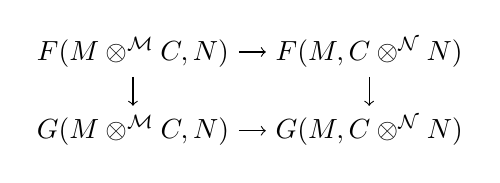
\begin{tikzpicture}
	\node (LT) at (0, 1) {$F(M \otimes^{\cM} C, N)$};
	\node (LB) at (0, 0) {$G(M \otimes^{\cM} C, N)$};
	\node (RT) at (3, 1) {$F(M, C \otimes^{\cN} N)$};
	\node (RB) at (3, 0) {$G(M, C \otimes^{\cN} N)$};
	\draw [->] (LT) -- node [left] {$$} (LB);
	\draw [->] (LT) -- node [above] {$$} (RT);
	\draw [->] (RT) -- node [right] {$$} (RB);
	\draw [->] (LB) -- node [below] {$$} (RB);
	%\node at (0.5, 1) {$\ulcorner$};
	%\node at (1.5, 0.5) {$\lrcorner$};
\end{tikzpicture}.
\end{center}
\end{definition}


\begin{definition}
	Let $\cA$ and $\cB$ be right and left $\cC$-module categories, respectively. The {\em Deligne tensor product $\cA \boxtimes_{\cC} \cB$} is the universal linear category admitting a $\cC$-balanced multilinear functor $\boxtimes_{\cC}: \cA \times \cB \to \cA \boxtimes_{\cC} \cB$. That is, there exists a $\cC$-balanced multilinear functor $\boxtimes_{\cC}: \cA \times \cB \to \cA \boxtimes_{\cC} \cB$ which induces, for all linear categories $\cD$, an equivalence between the categories of $\cC$-balanced multilinear functors $\cA \times \cB \to \cD$ and linear functors $\cA \boxtimes_{\cC} \cB \to \cD$. 
\end{definition}

If it exists, the Deligne tensor product is unique up to an equivalence, which in turn is unique up to unique natural isomorphism. Equivalently, the 2-category of linear categories representing the Deligne tensor product is either contractible or empty. 

\begin{theorem} \label{thm:DelignePrdtOverATCExists}
	Let $\cC$ be a finite rigid tensor category and let $\cA_{\cC}$ and ${}_{\cC}\cB$ be finite right and left $\cC$-module categories, respectively. Then,
	\begin{enumerate}
		\item The Deligne tensor product $\cA \boxtimes_{\cC} \cB$ exists and is a finite linear category;
		\item If $\cA = \Mod{A}{}(\cC)$ and $\cB = \Mod{}{B}(\cC)$, then $\cA \boxtimes_{\cC} \cB \simeq \Mod{A }{B}(\cC)$;

		\item The functor $\boxtimes_{\cC}$ is exact in each variable and satisfies 
		\begin{equation*}
			\Hom_{\cA}(x,x') \otimes \Hom_{\cB}(y, y') \cong \Hom_{\cA \boxtimes_{\cC} \cB} (x \boxtimes_{\cC} y, x' \boxtimes_{\cC} y'),
		\end{equation*}
		\item If $F: \cA \times \cB \to \cD$ is a $\cC$-balanced multilinear functor which is exact in each variable, then it defines an exact functor $\overline{F}: \cA \boxtimes_{\cC} \cB \to \cD$. 
	\end{enumerate} 
\end{theorem}

%\begin{remark} \label{rmk:rigidpreservedbytensor}
%	We may use the case $\cC= \Vect_k$ to rewrite part of the data of a tensor category as a linear category $\cD$ equipped with an object $1 \in \cD$ and a linear functor $\otimes: \cD \boxtimes \cD \to \cD $, together with natural transformations $\alpha$, $\lambda$, and $\rho$, as before. Moreover by Corollary \ref{cor:RigidityViaFunctors} the tensor product of two rigid tensor categories is again rigid. 
%\end{remark}

\begin{remark}
	If ${}_{\cD}\cA_{\cC}$ and ${}_{\cC}\cB_{\cE}$ are bimodule categories, then the actions of $\cD$ and $\cE$ induce a $\cD$-$\cE$-module category structure on $\cA \boxtimes_{\cC} \cB$. This bimodule category satisfies the analogous universal property for $\cC$-balanced twisted bilinear bimodule functors. 
\end{remark}

The following lemma is crucial for proving our results.

\begin{lemma} \label{Lma:FunctorsAsATensorPdt}
	If $\cC$ is a finite rigid tensor category and $\cM$ and $\cN$ are finite left $\cC$-module categories then the natural functor induces an equivalence
	\begin{equation*}
		\Fun_\cC(\cM, \cC) \boxtimes_\cC \cN \simeq \Fun_\cC(\cM,\cN).
	\end{equation*}
	Here $\Fun_\cC$ denotes the category of (right exact) $\cC$-module functors. 
	Moreover, if $\cM$ and $\cN$ are bimodule categories, then the above equivalence is a bimodule equivalence. 
\end{lemma}

\begin{proof}
	The last sentence follows since in that case the natural functor is a bimodule functor. By Theorem \ref{thm:EGNO2.11.6}, there exist algebra objects $A, B \in \cC$ and equivalences $\cM \simeq \Mod{}{A}(\cC)$ and $\cN \simeq \Mod{}{B}(\cC)$. We show that both sides of the above equation are naturally equivalent to $\Mod{A}{B}(\cC)$, the category of $A$-$B$-bimodule objects in $\cC$. The equivalence $\Fun_\cC(\cM, \cN) \simeq \Mod{A}{B}(\cC)$ (\cite[Prop 2.12.2]{EGNO}) can be seen by mirroring the classical proof. A bimodule clearly gives rise to such a functor, and given a functor $f$, we obtain an $A$-$B$-bimodule $f(A)$. By $\cC$-linearity $f(X \otimes A) \cong X \otimes f(A)  \cong (X \otimes A) \otimes_A f(A) $ is determined on free $A$-modules. Since every object of $\cM$ may be written as a (canonical) coequalizer of free $A$-modules,
	\begin{equation*}
		M \leftarrow M \otimes A \leftleftarrows M \otimes A \otimes A
	\end{equation*} 
the functor $f$ is equivalent to the one determined by the bimodule $f(A)$. Thus the natural map  $\Mod{A}{B}(\cC) \to \Fun_\cC(\cM, \cN)$ is essentially surjective. The above argument also shows it is fully-faithful, so that $\Fun_\cC(\cM, \cN) \simeq \Mod{A}{B}(\cC)$, which in particular shows $\Fun_\cC(\cM, \cC) \simeq \Mod{}{A}(\cC)$. Now the result follows from Theorem \ref{thm:DelignePrdtOverATCExists}.
%Tensoring a left $A$-module and a right $B$-module gives a canonical $\cC$-balanced bilinear functor 
%\begin{equation*}
%	T: \Mod{A}{}(\cC) \times \Mod{}{B}(\cC) \to \Mod{A}{B}(\cC). 
%\end{equation*}
%To complete the proof we must show this induces an equivalence,
%\begin{equation*}
%	\Mod{}{A}(\cC) \boxtimes_\cC \Mod{B}{}(\cC) \simeq \Mod{B}{A}(\cC).
%\end{equation*}
%When $\cC = \Vect$, this is classical. More generally we must show that the right-hand-side has the desired universal property. For this purpose let $F:\Mod{}{A}(\cC) \times \Mod{B}{}(\cC) \to \cA$ be a $\cC$-balanced bilinear functor. There is a unique right exact linear functor $\overline F: \Mod{B}{A}(\cC) \to \cA$ such that $F = \overline{F} \circ T$ which is defined as follows. On free bimodules $A \otimes X \otimes B \cong T(A \otimes X, B)$, we necessarily have $\overline{F}(A \otimes X \otimes B) \cong F(A \otimes X, B)$. Since $\overline{F}$ is right exact and every $A$-$B$-bimodule is a coequalizer of free $A$-$B$-bimodules, the result follows. 	
\end{proof}

\begin{remark} \label{remark-tensorasfunctors}
If $\cM$ and $\cN$ are right $\cD$-modules, then we have that $\cN \boxtimes_\cD \Fun_{\cD}(\cM,\cD) \simeq \Fun_{\cD}(\cM,\cN)$, and again if $\cM$ and $\cN$ are bimodule categories, then this equivalence is a bimodule equivalence. 
\end{remark}

%%%%%%%%%

The following result is well-known, but we were unable to find a proof in the literature.

\begin{lemma} 
	Let $\cC$ be a rigid tensor category. Then every lax (respectively oplax) $\cC$-module functor is strong. This holds even if the functor is not right exact.   
\end{lemma}

\begin{proof}
We do the oplax case, the lax case is similar.  Suppose that $f_{c,m}:  c \otimes \cF(m) \rightarrow \cF(c \otimes m)$ is a binatural transformation making $\cF$ into an oplax module functor.  The inverse to this natural transformation is given explicitly by the mate of $f_{c^*,m}$ 
$$\cF(c \otimes m) \rightarrow c \otimes c^* \otimes \cF(c \otimes m) \rightarrow c \otimes \cF(c^* \otimes c \otimes m) \rightarrow c \otimes \cF(m)$$
where the first map is given by the coevaluation, the second map is $f_{c^*,m}$, and the third map is evaluation.

\NScomm{[Insert diagram here]}

We need to check that this map is inverse to $f_{c^*,m}$.  This is a straightforward calculation, first use the associativity condition for module functors, and second use naturality to pull an evaluation through the natural transformation.  The following diagram illustrates this calculation.

\NScomm{[Insert diagram here]}
\end{proof}


\begin{lemma} \label{lma:module-adjoint}
Let $\cC$ and $\cD$ be rigid tensor categories. Let  $\cM$ and  $\cN$  be  $\cC$-$\cD$-bimodule categories and let $\cF: \cM \to \cN$ be a $\cC$-$\cD$-bimodule functor.  If the underlying functor of $\cF$ has a right (respectively left) adjoint as a functor, then $\cF$ has a right (resp. left) adjoint $\cC$-$\cD$-bimodule functor. 
\end{lemma}
\begin{proof}
Suppose that $\cG$ is the right adjoint to the underlying functor of $\cF$, we will show that $\cG$ has a natural structure of a $\cC\boxtimes \cD^{mp}$-module functor.  The result for left adjoints is similar.

The binatural transformation $\psi_{x,n}: x \otimes \cG(n) \rightarrow \cG(x \otimes n)$ is given by the mate
$$x \otimes \cG(n) \rightarrow \cG \cF(x \otimes \cG(n)) \rightarrow \cG(x \otimes \cF\cG(n)) \rightarrow \cG(x \otimes n)$$
where the first map is the unit of the adjunction, the second map is the binatural transformation coming from the module functor structure on $\cF$ and the third map is the counit.  (Note that this mate rotates in the opposite direction from the one in the previous lemma.)

\NScomm{[Insert diagram here]}

Applying the previous lemma, rigidity of $\cC$ and $\cD$ guarantees that this binatural transformation is an isomorphism.  The compatibility condition is an easy exercise with commuting diagrams.
\end{proof}

\begin{remark}
If $\cC$ and $\cD$ are not rigid the above argument only shows that the right adjoint to a (lax) module functor has an oplax module functor structure, while the left adjoint of an (oplax) module functor only has a lax module functor structure.  This is a serious issue as the following example shows. 
\end{remark}

\begin{example} \label{ex:lax-module}

	Let $\cR \cong \Vect \oplus \Vect \cdot X$ be the non-rigid tensor category consisting of pairs of vector spaces, which we write as $V_1 + V_2 X$, with tensor product given by 
	\begin{equation*}
		(V_1 + V_2 X) \otimes (W_1 + W_2 X) = V_1 \otimes V_2  +  (V_1 \otimes W_2 \oplus V_1 \otimes W_1)X.
	\end{equation*} 
	Up to equivalence there are unique choices of associator and unitors making this tensor category. It is a categorification of the ring $k[x]/(x^2)$ as a finite semisimple tensor category, but it is not rigid. The object $X$ cannot have a dual as there is no object $Z \in \cR$ such that $Z \otimes X$ has a non-zero map to or from the unit object of $\cR$. 
	
	There is a tensor functor $F:\cR \to \Vect$ given by $(V_1 + V_2 X) \mapsto V_1$. This gives the category $\Vect$ the structure of a (left) $\cR$-module category, and moreover $F$ is naturally an $\cR$-module map. $F$ has both a left and right adjoint, which agree and are given by the functor $G: \Vect \to \cR$ sending $W \in \Vect$ to $(W + 0 X) \in \cR$. It is not possible to give $G$ the structure of an $\cR$-module functor. 
\end{example}


For rigid tensor categories, it will sometimes be convenient to have an alternative description of $\Fun_C(\cM,\cC)$.

\begin{definition}
Let ${}^*\cM$ denote the $\cD$--$\cC$ bimodule category whose underlying category is $\cM^{\op}$ and the action is given by $d\cdot m \cdot c = {}^*c \otimes m \otimes {}^*d$.  Similarly, let $\cM^*$ denote the $\cD$--$\cC$ bimodule category whose underlying category is $\cM^{\op}$ and the action is given by $d\cdot m \cdot c = c^* \otimes m \otimes d^*$.  
\end{definition}

\begin{lemma}
If ${}_{\cC}\cM_\cD$ is a $\cC$-$\cD$ bimodule category and ${}_{\cC}\cN_\cE$ is a $\cC$-$\cE$ bimodule category, then taking right adjoints gives an equivalence of $\cD$-$\cE$ bimodules $\Fun_{\cC}(\cM, \cN)$ and $\Fun^L_{\cC}(\cN, \cM)^*$ where $\Fun^L_\cC$ denotes {\em left exact} $\Vect$-enriched module functors.  Similarly, if $\cM$ is a $\cC$-$\cD$ bimodule category and $\cN$ is a $\cD$-$\cE$ bimodule category, then taking right adjoints gives an equivalence of $\cC$-$\cE$ bimodules ${}^*\Fun_{\cD}(\cM, \cN) \rightarrow \Fun^L_{\cD}(\cN, \cM)$. 
\end{lemma}
\begin{proof}
	We will prove the first statement as the second follows from a nearly identical argument. 
We've already seen in Lemma \ref{lma:module-adjoint} that the adjoint of a module functor has a canonical module functor structure.  Furthermore, taking left adjoints is clearly an equivalence of the relevant functor categories; the inverse equivalence is given by taking right adjoints. Thus we need only check that the $\cD$-$\cE$ bimodule structures agree under this equivalence.  First note that taking adjoints reverses the order of composition. Secondly the right adjoint of right multiplication by $x$ is right multiplication by $x^*$, while in the latter case we have that the right adjoint of left multiplication by $x$ is left multiplication by ${}^*x$.
\CSP{This needs tending and I think there is an error here.}
\NS{I fixed the error, but feel free to do more tending.}
\end{proof}

\begin{lemma} \label{lem:dual-formula-for-adjoints}
We have that ${}^*\cM \cong \Fun_{\cD}(\cM, \cD)$ and $\cM^* \cong \Fun_{\cC}(\cM, \cC)$.
\end{lemma}
\begin{proof}
By the previous lemma, $\Fun_{\cC}(\cM, \cC) \cong \Fun_{\cC}^L(\cC, \cM)^*$  But the latter is just $\cM^*$ since any module functor $\cF$ from $\cC$ to $\cM$ is right multiplication by $\cF(1)$.
\end{proof}

\begin{remark}
Combining Lemmas \ref{lem:dual-formula-for-adjoints} and \ref{Lma:FunctorsAsATensorPdt} we have that if $\cM$ is a finite rigid $\cD$-$\cC$ bimodule and $\cN$ is a finite rigid $\cC$-$\cE$ bimodule, then $\cM \boxtimes_\cC \cN \cong ({}^*\cM)^* \boxtimes_\cC \cN \cong \Fun_{\cC\text{-mod}}({}^*\cM,\cN)$ as $\cD$-$\cE$ bimodule categories.   Similarly, $\cM \boxtimes_{\cC} \cN \cong \cM \boxtimes_\cC {}^*(\cN^*) \cong \Fun_{\text{mod-}\cC}(\cN^*,\cM)$ as $\cD$-$\cE$ bimodule categories.  These bimodule category isomoprhisms are the correct version of \cite[Remark 3.6]{0909.3140} which was originally incorrect as stated for bimodule categories.
\end{remark}


\subsection{Exact module categories and adjoints of module functors}
Throughout this section we consider only finite rigid tensor categories.  The goal of this section is to summarize Etingof and Ostrik's theory of exact module categories \cite{MR2119143}.  The goal is to be able to show that certain module functors have adjoints in proving $3$-dualizability.

\begin{definition}
	Let $\cC$ be a finite rigid tensor category. A (left) $\cC$-module category $\cM$ will be called {\em exact} if for any object $M \in \cM$ and  projective object $P \in \cC$, the object $P \otimes M$ is projective in $\cM$. 
\end{definition}

\begin{example}
	If $\cC$ is semisimple (e.g. $\cC = \Vect$), then $\cM$ is an exact module category if and only if it is also semisimple.
\end{example}

\begin{example}[{\cite[Example 2.6.5]{EGNO}}]
	The finite rigid tensor category $\cC$ is exact considered as a $\cC$-, $\cC^{mp}$-, or $\cC \otimes \cC^{mp}$-module category. 
\end{example}

The following omnibus theorem summarizes the key properties of exact module categories: 
\begin{theorem}[ \cite{EGNO}] \label{Thm:ExactModCatOmnibus}
	Let $\cC$ be a finite rigid tensor category, and let $\cM$, $\cM'$, $\cM''$ be exact $\cC$-module categories, and $\cN$ an arbitrary $\cC$-module category. Then,
	\begin{enumerate}
		\item $\cM$ has enough projectives \cite[Lemma 2.7.1]{EGNO}
		\item Every projective object in $\cM$  is injective, and vice versa. \cite[Cor 2.7.4]{EGNO}
		\item $\Fun_{\cC}(\cM, \cM')$ is finite \cite[Prop 2.13.5]{EGNO}; In particular $\cM \simeq \Fun_{\cC}(\cC, \cM)$ is finite.
		\item Composition $\Fun_{\cC}(\cM, \cM') \times \Fun_{\cC}(\cM', \cM'') \to \Fun_{\cC}(\cM, \cM'')$ is exact in each variable. \cite[Lemma 2.13.2]{EGNO}		
		\item Every additive (not a priori right exact) module functor $F:\cM \to \cN$ is exact \cite[Prop 2.7.8]{EGNO}. Hence every functor $F \in \Fun_{\cC}(\cM, \cM')$ is exact, and has exact left and right adjoints. Moreover, it follows that   $\Fun_{\cC}(\cM,\cM)$ is again a finite rigid tensor category. 
	\end{enumerate}
\end{theorem}


\subsection{Separability} \label{sec-tc-separable}
In characteristic $0$, fusion categories and their semisimple bimodule categories have many good closure properties.  For example, M\"uger's proves that the Drinfel'd center  of a fusion category is fusion \cite[Theorem 3.16]{MR1966525} and Etingof--Nikshych--Ostrik's show that functor categories between semisimple module categories over fusion categories are semsimple and hence semisimplicity is preserved by relative Deligne tensor product \cite[Theorem 2.16]{MR2183279}.  However, it is well-known that these results break down non-zero characteristic.  This happens for two separate reasons, first fusion categories of global dimension $0$ behave poorly, and second (as observed by Kuperberg \cite[Question 5.1]{MR1995781}) if you work over a non-perfect field there are some problems related to inseparable field extensions.

In this section, we introduce a new notion of separability for algebra objects, module categories, and tensor categories which provides the right setting for generalizing the results of M\"uger and Etingof--Nikshych--Ostrik to characteristic $p$.  This theory is a generalization of the classical notion of a separable algebra \cite{???}.   This section was inspired by a suggestion of Ostrik, and by the appearance of separability in the classification of $2$-dimensional local field theories \cite{schommer-pries-thesis}.

\begin{definition}
	Let $A$ be an algebra object in a finite tensor category $\cC$. The multiplication map $\mu: A \otimes A \to A$ may be viewed as a morphism of $A$-$A$-bimodule objects in $\cC$. We will say that $A$ is {\em separable} if the multiplication map splits as a map of $A$-$A$-bimodules. 
\end{definition}

\begin{remark}
	A (right exact) monad $T$ acting on a $\cC$-module category $\cM$ is an algebra object in the tensor category $\Fun_\cC(\cM, \cM)$. Thus the above definition also yields the notion of {\em separable monad}. 
\end{remark}

\begin{remark}
	When $\cC = \Vect_k$, then a separable algebra $A$ is separable in the classical sense. Over a perfect field --- such as a finite field, an algebraically closed field, or a field of characteristic zero --- this is equivalent to $A$ being a finite dimensional semisimple $k$-algebra; more generally it is a stronger condition. 
	\CSP{get references to classical notion of separability}
\end{remark}

\begin{theorem} \label{thm:SepModCats}
	Let $\cC$ be a finite semisimple tensor category and let $\cM$ be a finite right $\cC$-module category. Then the following are equivalent:
	\begin{enumerate}
		\item $\cM_\cC \simeq \Mod{A}{}(\cC)$, where $A$ is a separable algebra in $\cC$;
		\item $\cM_\cC \simeq \Mod{A}{}(\cC)$, where $A$ is an algebra in $\cC$ which is projective as an $A$-$A$-bimodule;
		\item The identity functor is a projective object of $\Fun_\cC(\cM, \cM)$;
		\item $\Fun_\cC(\cM, \cM)$ is a semisimple category. 
	\end{enumerate}
	Moreover if any of these conditions is satisfied, then $\cM$ is semisimple, hence exact as a $\cC$-module category. The analogous results hold for left $\cC$-module categories as well. 
\end{theorem}


\begin{proof}
	The last sentence is clear since we may switch left/right actions by taking the monoidally-opposite category.
	The proof of Lemma \ref{Lma:FunctorsAsATensorPdt} shows that $\Fun_\cC(\cM, \cM) \simeq \Mod{A}{A}(\cC)$, thus we have clear implications (4) $\Rightarrow$ (3) $\Leftrightarrow$ (2) $\Rightarrow$ (1). We will show that (1) $\Rightarrow$ (4), that is if $A$ is separable, then $\Mod{A}{A}(\cC)$ is a semisimple category. 
	
	To see this, recall the following general fact: if $F: \cA \leftrightarrows \cB: G$ is an adjunction between abelian categories and the right adjoint $G$ is also right exact, then $F$ sends projective objects to projective objects. This is clear as
	\begin{equation*}
		\Hom(F(P), -) \cong \Hom(P, U(-))
	\end{equation*}
	is a right-exact functor. In particular this applies to the free-forget adjunction between $A$-$A$-bimodules and objects of $\cC$. As every object of $\cC$ is projective (since it is semisimple) we have that every free $A$-$A$-bimodule is also projective in $\Mod{A}{A}(\cC)$. 
	
Let $s: {}_AA_A \to {}_AA \otimes A_A$ be a bimodule splitting of the multiplication map. For every $A$-$A$-bimodule $X$ we have an induced $A$-$A$-bimodule map
\begin{equation*}
	X \cong A \otimes_A X \otimes_A A 
	\xra{s \otimes_A 1 \otimes_A s} (A \otimes A) \otimes_A X \otimes_A (A \otimes A) \cong A \otimes X \otimes A,
\end{equation*}  	
which splits the canonical action map. Thus $X$ is a direct summand of the free bimodule $A \otimes X \otimes A$. As this latter is projective, $X$ is projective. Thus $\Mod{A}{A}(\cC)$ is semisimple, and (1) $\Rightarrow$ (4). 
	
Similarly if $Y \in \cM \simeq \Mod{A}{}(\cC)$ is a left $A$-module, then $s \otimes_A 1: Y \cong A \otimes_A Y \to (A \otimes A) \otimes_A Y \cong A \otimes Y$ realizes $Y$ as a direct summand of a free $A$-module. Again since $\cC$ is semisimple, free $A$-modules are necessarily projective. Thus $Y$ is projective. Hence $\cM$ itself is semisimple.  	
\end{proof}

\begin{definition}
	If any of the equivalent conditions of Theorem \ref{thm:SepModCats} are satisfied, then we will say that $\cM$ is a {\em separable} module category. If $\cM$ is a $\cC$-$\cD$-bimodule category then we will say $\cM$ is separable if it is separable over both $\cC$ and $\cD$ separately. 
\end{definition}

A linear category $\cC$ is a $\Vect$-separable if and only if it can be realized as a category of algebras over a separable algebra.  Thus $\Vect$-separability is well-understood.   $\Vect$-separability implies semisimplicity, and over a perfect field it is equivalent to semisimplicity.  More generally, each simple object $X$ in a semisimple category $\cC$ has a division ring of endomorphisms $D_X$ with center $K_X$, and $\cC$ is separable if and only if $K_X/k$ is a separable field extension.  Equivalently, a linear category is $\Vect$-separable if and only if it is absolutely semisimple in the sense that the category remains semisimple under arbitrary base changes.  Since the word ``separable" is somewhat overloaded in this section we will say absolutely semisimple instead of $\Vect$-separable.

\begin{theorem} \label{thm:compositeOfSep}
	If ${}_\cB\cM_\cC$ and ${}_\cC\cN_\cD$ are separable bimodule categories over semisimple tensor categories, then $\cM \boxtimes_{\cC} \cN$ is a separable $\cB$-$\cD$-bimodule category.
\end{theorem}

\begin{proof}
	As separability is a condition on each module structure separately, is is enough to check that $\cM \boxtimes_{\cC} \cN$ is a separable as a $\cB$-module category. Our assumptions give the following identifications:
\begin{itemize}
	\item $\cM \simeq \Mod{}{A}(\cB)$ as left $\cB$-module categories for a separable algebra $A$ in $\cB$;
	\item $\cM \simeq \Mod{B}{}(\cC)$ as right $\cC$-module categories for a separable algebra $B$ in $\cC$;
	\item $\cN \simeq \Mod{}{C}(\cC)$ as left $\cC$-module categories for a separable algebra $C$ in $\cC$;
	\item $\cM \boxtimes_{\cC} \cN \simeq \Mod{B}{C}(\cC)$
\end{itemize}
Thus $\cM \boxtimes_{\cC} \cN$ is equivalent to the category of algebras for the separable monad $T = (-) \otimes C$ acting on $\cM$. Moreover $T$ is an algebra (monad) in $\Fun_{\cB}(\cM, \cM)$ (this follows as the left $\cB$-action on $\cM$ commutes up to coherent natural isomorphism with the right $\cC$-action), and this induces the structure of an algebra on the object $T(A) \in \cB$. The multiplication is given by,
\begin{equation*}
	T(A) \otimes T(A)  \simeq T( T(A) \otimes A)  \xra{T(\textrm{action})} T^2(A) \to T(A),
\end{equation*}
where the first equivalence comes from left $\cB$-linearity of $T$, the next map comes from the action map on $T(A)$ ($T(A) \in \cM \simeq \Mod{}{A}(\cB)$ has a right $A$-action), and the final map is one of the structure maps of the monad $T$. The unit of $T(A)$ is defined similarly. 

One readily verifies that the the unit map $A \to T(A)$ is an homomorphism of algebras in $\cB$. Moreover as $T$ is right exact and $\cB$-linear, we have $T(m) \cong m \otimes_A T(A)$ for all $m \in \Mod{}{A}(\cB) \simeq \cM$. Thus the category of $T$-algebras in $\Mod{}{A}(\cB)$ is nothing more then the category of right $T(A)$-modules in $\cB$.  Hence we have shown $\cM \boxtimes_{\cC} \cN \simeq \Mod{}{T(A)}(\cB)$ as left $\cB$-module categories. It remains to show that $T(A)$ is a separable algebra in $\cB$.

As both $A$ and $T$ are separable, we have splittings of the canonical multiplication maps, $s: A  \to A \otimes A$, and $\sigma:T \to T^2$. These induce a splitting of the $T(A)$-multiplication map:
\begin{equation*}
	T(A) \stackrel{\sigma}{\to} T^2(A) \xra{T(1 \otimes_A s)} T( T(A) \otimes A) \cong T(A) \otimes T(A).
\end{equation*}
Thus $T(A)$ is separable.
\end{proof}

$\cC$ is always seperable as a $\cC$-$\cC$ bimodule category.  However, we will often need to consider $\cC$ as a $\cC \boxtimes \cC^\mp$-$\Vect$ as well.  This suggests the following definition.

\begin{definition}
	A semisimple tensor category is {\em separable} if it is separable as a $\cC \boxtimes \cC^\mp$-$\Vect$-bimodule category.  
\end{definition}


\begin{definition}
	Let $\cC$ be a finite tensor category. The {\em center} of $\cC$ is the linear category $\cZ(\cC) \simeq \Fun_{\cC \boxtimes \cC^\mp}(\cC, \cC)$.
\end{definition}

\begin{corollary}
	The following are equivalent for an absolutely semisimple finite tensor category $\cC$.
	\begin{enumerate}
		\item $\cC$ is separable;
		\item The center $\cZ(\cC)$ is semisimple.
	\end{enumerate} 
\end{corollary}

\begin{theorem}
Separable finite tensor categories, finite absolutely semisimple separable bimodule categories, bimodule functors, and bimodule natural transformations, form a symmetric monoidal $3$-subcategory of $\TC$.
\end{theorem}
\begin{proof}
This follows from applying the previous theorem a bunch of times.  $\Vect$ separability of the bimodule categories is needed for the monoidal structure
\end{proof}


\subsection{Fusion categories} \label{sec-tc-fusion}.%!%remove period

The goal of this section is to show that under nice circumstances separability is easy to check.  In particular, we show that over an algebraically closed field fusion categories of nonzero global dimension are separable, and that semisimple bimodule categories over such fusion categories are separable.  In this section we do not strive for generality, but instead have the practical aim of showing that separability is easy to check for examples.

For the entirety of this section the base field $k$ will be algebraically closed.  Recall that a tensor category over an algebraically closed field is called fusion if it is semisimple rigid finite and the trivial object is simple.  In such a setting there's a well-defined notion of global dimension.  It is well-known \cite{???}, that over an algebraically closed field non-zero global dimension implies that $\cZ(\cC)$ is semisimple and hence $\cC$ is separable.  We quickly sketch a proof of a stronger version of this result which was suggested to us by Victor Ostrik.

\begin{theorem} \label{thm:NonzeroDimension}
A fusion category $\cC$ is seperable if and only if its global dimension is non-zero.
\end{theorem}
\begin{proof}
We first prove that global dimension non-zero implies separability.  Let $A \in \cC \boxtimes \cC^\mp$ be the algebra of internal endomorphisms of the identity object in $\cC$.  This algebra can be described explicitly, as an object it is $\bigoplus_X X \boxtimes {}^*X$.  This algebra has a Frobenius algebra structure given by the trace given by projection onto the $1 \boxtimes 1$ component.  The comultiplication for this Frobenius algebra gives a bimodule map $\Delta: {}_A A_A \rightarrow {}_A A \otimes A_A$.  The composition $m \circ \Delta$ is exactly the global dimension of $\cC$.  Hence, if the global dimension is nonzero then $A$ is seperable.

In the other direction, note that if $\cC$ is separable then the category of $A$-$A$ bimodules is semisimple.  The space of $A$-$A$ bimodule maps from $A \otimes A$ to $A$  is $1$-dimensional, and hence by semisimplicity, there's also a $1$-dimensional space of maps the other direction.  In particular, any bimodule map $A \otimes A \rightarrow A$ is a multiple of $\Delta$.  Since separability says that there's some splitting of multiplication, this splitting must be some multiple of $\Delta$ and so can only exist if $\Delta$ gives such a splitting, that is to say that the global dimension is nonzero.
\end{proof}


\begin{theorem} \label{thm:SSModuleCatsAreSep}
If $\cC$ is fusion and $\cM$ is a semisimple module category over $\cC$, then $\cM$ is separable.
\end{theorem}
\begin{proof}
It is easy to reduce to the case where $\cM$ is indecomposable.  Then, by \cite{???}, there is a surjective tensor functor $Z(\cC) \rightarrow \Fun_\cC(\cM, \cM)$.  Thus, by \cite{???}, $\Fun_\cC(\cM, \cM)$ is semisimple and $\cM$ is separable.
\end{proof}

It would be nice to give a more direct proof of Theorem \ref{thm:SSModuleCatsAreSep} following the proof of Theorem \ref{thm:NonzeroDimension} .  It's easy to get an algebra with trace, but it was not clear to us why the resulting bilinear form is nondegenerate.  By contrast in the setting of Theorem \ref{thm:NonzeroDimension} we have a concrete formula for the bilinear form.


\section{Local field theory in dimension three} \label{sec-lft}

\CDcomm{[Insert a few introductory sentences here, including a statement of the cobordism hypothesis.  That will motivate the need for a notation of n-framed manifolds, and for describing various structure groups.  Then we can forward reference to 3.2 the more detailed discussion of the cobordism hypothesis.]}

\CD{Somewhere, presumably in section 3, add the picture with the series of adjoints of cups and caps with twists.}

\subsection{Notation for $n$-framed manifolds} 

Since $n$-framed manifolds play a fundamental role in the cobordism hypothesis it will be important to have convenient notation to denote $n$-framed manifolds.  We describe one such notation involving immersions in this section.

Recall that by definition an $n$-framed $k$-manifold $(M,\tau)$ is a k-manifold $M$ equipped with a trivialization $\tau$ of $TM \oplus \RR^{n-k}$.  A convenient way to specify an $n$-framing on a $k$-manifold is to give an immersion $\iota: M \hra \RR^n$ together with a framing $\phi$ of the normal bundle of this immersion.  The framing $\phi$ is by definition an ordered collection of $n-k$ orthonormal sections of the normal bundle $\nu(\iota)$; this framing can equivalently be viewed as a trivialization $\phi: \nu(\iota) \simeq \RR^{n-k}$ of the normal bundle.  The normally framed immersion $(\iota, \phi)$ provides an $n$-framing on $M$ by the composite
\[TM \oplus \RR^{n-k} \simeq TM \oplus \nu(\iota) \simeq  \RR^n.\]
Here the first isomorphism is provided by the inverse of the normal framing $\phi$, and the second isomorphism is given by the standard (``blackboard") identification of the sum of the tangent bundle and the normal bundle with the trivial bundle.

When drawing $n$-framed manifolds using the normally framed notation described above, we draw the immersed manifold and draw the normal framing, and leave the induced $n$-framing completely implicit.  When the immersion is codimension-1, the normal framing may be indicated simply by a unidirectional gray corona coming off the manifold.  Moreover, because in the codimension-1 case this corona can propagate without ambiguity, it may be indicated only at one point of the manifold.

\begin{example}
Let $M$ be a closed connected 2-framed 1-manifold.  By definition $M$ comes equipped with a bundle isomorphism $\phi: TM \oplus \RR \xra{\simeq} \RR^2$. Let $\iota$ denote the orientation of $M$ such that for any point $p \in M$, the pair $(\phi_p(\iota,0),\phi_p(0,1))$ is a positive frame of $\RR^2$.  This orientation provides another 2-framing of $M$, namely $\omega: TM \oplus \RR \xra{\iota \oplus \id} \RR^2$.  The ratio $\phi/\omega$ is a map $M \ra SO(2)$.  Because $M$ is oriented, the homotopy classes of such maps is the integers.  We therefore have a $\ZZ$-valued invariant of closed 2-framed 1-manifolds, and in fact this procedure produces an isomorphism from the 2-framed diffeomorphism classes of closed connected 2-framed 1-manifolds to the integers.  We use our immersion notation to depict, as follows, a series of circles corresponding to each 2-framed diffeomorphism class:
\[\cdots\quad
\cb{
\begin{tikzpicture}
{ [xshift=-3cm]
\draw[linestyle,fuzzleft]
(.5,0) to [out=-90, in=25] (.3,-.3)
	to [looseness=1.6, out=-155, in=225] (.15,-.15)
	to [looseness=1.6, out=45, in=65] (.3,-.3)
	to [out=245, in=-65] (-.3,-.3)
	to [looseness=1.6, out=115, in=135] (-.15,-.15)
	to [looseness=1.6, out=-45, in=-25] (-.3,-.3)
	to [out=155, in=-90] (-.5,0)
	.. controls (-.5,.66) and (.5,.66) .. (.5,0);	
}
{ [xshift=-1.5cm]
\draw[linestyle,fuzzleft]
(.5,0) to [out=-90, in=-20] (0,-.4)
	to [looseness=1.6, out=160, in=180] (0,-.1)
	to [looseness=1.6, out=0, in=20] (0,-.4)
	to [out=-160, in=-90] (-.5,0)
	.. controls (-.5,.66) and (.5,.66) .. (.5,0);
}
{ [xshift=0cm]
\draw[linestyle,fuzzleft]
(.5,0) .. controls (.5,-.66) and (-.5,-.66) .. (-.5,0)
	.. controls (-.5,.66) and (.5,.66) .. (.5,0);
}
{ [xshift=1.5cm]
\draw[linestyle,fuzzleft,looseness=2]
(0,.5) to [out=0, in=10] (0,0)
	to [out=-170, in=180] (0,-.5)
	to [out=0, in=-10] (0,0)
	to [out=170, in=180] (0,.5);
}
{ [xshift=3cm]
\draw[linestyle,fuzzright]
(.5,0) .. controls (.5,-.66) and (-.5,-.66) .. (-.5,0)
	.. controls (-.5,.66) and (.5,.66) .. (.5,0);
}
{ [xshift=4.5cm]
\draw[linestyle,fuzzright]
(.5,0) to [out=-90, in=-20] (0,-.4)
	to [looseness=1.6, out=160, in=180] (0,-.1)
	to [looseness=1.6, out=0, in=20] (0,-.4)
	to [out=-160, in=-90] (-.5,0)
	.. controls (-.5,.66) and (.5,.66) .. (.5,0);
}
{ [xshift=6cm]
\draw[linestyle,fuzzright]
(.5,0) to [out=-90, in=25] (.3,-.3)
	to [looseness=1.6, out=-155, in=225] (.15,-.15)
	to [looseness=1.6, out=45, in=65] (.3,-.3)
	to [out=245, in=-65] (-.3,-.3)
	to [looseness=1.6, out=115, in=135] (-.15,-.15)
	to [looseness=1.6, out=-45, in=-25] (-.3,-.3)
	to [out=155, in=-90] (-.5,0)
	.. controls (-.5,.66) and (.5,.66) .. (.5,0);	
}
\end{tikzpicture}
}
\quad \cdots
\]

\end{example}

\begin{warning}  \NS{What about in nonzero codimension?  Is there a theorem saying those always come from immersions?}
Not every $n$-framed $n$-manifold can be specified in this way. For example the circle has no immersion into $\RR^1$ but does have a (unique) $1$-framing.
\end{warning}

For $m < n$, an $m$-framed $k$-manifold $(M,\tau)$ is naturally $n$-framed by the trivialization $\tau \oplus \gamma$ where $\gamma$ is the canonical trivialization of $\RR^{n-m}$.  Similarly, given a normally framed immersion $(\iota: M \hra \RR^m, \phi: \nu(\iota) \simeq \RR^{m-k})$, there is a naturally associated normally framed immersion $(M \hra \RR^m \ra \RR^n, \phi \oplus \id_{\RR^{n-m}})$.  This stabilization of a normally framed immersion is clearly compatible with the stabilization of the associated $m$-framed manifold.

\begin{example}
The unique $1$-framing on the circle induces a $2$-framing on the circle; that $2$-framing agrees with the $2$-framing induced by the figure 8 immersion above. 
\end{example}

The association of an $n$-framed manifold to a normally framed immersion works just as well for manifolds with boundary or manifolds with corners.  Moreover, when these manifolds are bordisms, we can fix conventions for how a normal framing (therefore $n$-framing) of the bulk induces a normal framing (therefore $n$-framing) of the boundary.  Given a bordism $M$ without corners, each boundary component of $M$ is labelled either ``in" or ``out", according to whether it is part of the source or target of the bordism.  Now suppose $M$ is equipped with a normally framed immersion $(\iota,\phi)$.  An incoming boundary component $N \subset (\partial M)_{\textrm{in}}$ inherits the structure of a normally framed immersion: the immersion is the restriction of the immersion of $M$, and the framing is $(j, s) \subset \nu(N,\RR^n)$, where $j$ is a section of the normal bundle of $N$ pointing into the bulk manifold $M$, and $s \subset \nu(M,\RR^n)$ is the given normal frame of $M$.  Given a higher bordism, that is a manifold $M$ with corners representing a morphism in $\Bord_0^n$, that is equipped with a normally framed immersion, the incoming and outgoing boundaries (which are now codimension zero submanifolds of the boundary of $M$) inherit normal framings exactly as for the boundaries of ordinary bordisms.  Furthermore, the boundaries of these boundaries inherit normal framings by the same procedure.  Iterating this procedure for inducing normal framings on the boundaries provides consistently defined normal framings to every corner of the original bordism $M$.

In drawing manifolds with boundary and corners, we also need to specify which parts of the boundary are incoming and outgoing.  Outgoing pieces of the boundary will be indicated by a small arrow pointing out of the bulk of the manifold; incoming pieces of the boundary will be undecorated---implicitly the arrows would point into the bulk.  When the immersion is codimension zero, the outgoing boundary arrows may be replaced by a gray corona, which serves to directly record the induced normal framing of those parts of the boundary.  At corners, a combination of these indications will be used.  For instance, an arrow together with a corona on a codimension 2 corner indicates respectively the first and second vectors of the induced framing on the corner.

\begin{warning}
If $M$ is an $n$-manifold with boundary immersed in $\RR^n$ the corona indicates which boundaries are outgoing, while if $M$ is an $n-1$ manifold with boundary immersed in $\RR^n$ the corona indicates the trivialization of the normal bundle.  These two usages are compatible: the induced trivialization of the normal bundle of the outgoing boundary is indeed the outward trivialization, therefore indicated by an outward corona.  By contrast, the trivialization of the normal bundle of an incoming boundary is the inward trivialization, therefore would be indicated by a corona pointing into the bulk manifold; this type of corona is covered by the bulk and therefore cannot be seen.
\end{warning}

\begin{example} \label{eg-framenot0}
The following four pictures specify respectively a $0$-framed, a $1$-framed, and two $2$-framed 0-manifolds:
\[
\begin{tikzpicture}
\filldraw (0,0) circle (\pointrad);
\filldraw (1,0) circle (\pointrad); 
\begin{pgfonlayer}{background}
\draw[->,outstyle] (1,0) -- +(-\arrowlength,0);
\end{pgfonlayer}
\filldraw (2,0) circle (\pointrad);
\begin{pgfonlayer}{background}
\draw[->,outstyle] (2,0) -- +(45:\arrowlength) node[anchor=south,inner sep=2pt] {\tiny 1};
\draw[->,outstyle] (2,0) -- +(135:\arrowlength) node[anchor=south,inner sep=2pt] {\tiny 2};
\end{pgfonlayer}
\filldraw (3,0) circle (\pointrad); 
\begin{pgfonlayer}{background}
\draw[->,outstyle] (3,0) -- +(45:\arrowlength) node[anchor=south,inner sep=2pt] {\tiny 2};
\draw[->,outstyle] (3,0) -- +(135:\arrowlength) node[anchor=south,inner sep=2pt] {\tiny 1};
\end{pgfonlayer}
\end{tikzpicture}
\]
\end{example}

\begin{example}
Here is a picture of a $1$-framed manifold:
\[
\begin{tikzpicture}
\draw[linestyle] (0,0) -- (1.5,0);
\begin{pgfonlayer}{background}
\draw[->,outstyle] (0,0) -- +(180:\arrowlength);
\end{pgfonlayer}
\end{tikzpicture}
\] \CD{Notice that the arrow looks clipped here.  That is because tikzexternalize isn't adding enough margin when it creates pdf, or some such.  This problem will go away when we stop externalizing, and in any case should not be fixed by changing the arrows themselves.}
The right point is incoming, and the left point is outgoing.  Both boundary points inherit framings isomorphic to the second picture in example~\ref{eg-framenot0}.  Here is a picture of a $2$-framed manifold:
\[
\begin{tikzpicture}
\draw[linestyle,fuzzleft] 
(0,0) .. controls (1.1,1.1) and (1.25,.65) .. (1.25,.5)
	.. controls (1.25,.25) and (.875,.25) .. (.875,.5)
	.. controls (.875,.9) and (1.875,.9) .. (1.875,.5)
	.. controls (1.875,.25) and (1.5,.25) .. (1.5,.5)
	.. controls (1.5,.65) and (1.65,1.1) .. (2.75,0);
\end{tikzpicture}
\]
Both boundary points are incoming, and the induced framing on these points are, left to right, respectively the last two points pictured in example~\ref{eg-framenot0}.  Note that corona in this example specifies the trivialization of the normal bundle.
\end{example}

\begin{example}
Here is a picture of a $2$-framed manifold:
\[
\begin{tikzpicture}
\filldraw[linestyle,fuzzright,fill=\fillcolor] (0,0) circle (\circlerad);
\end{tikzpicture}
\]
Note that here the corona denotes that the boundary is outgoing.  This boundary is the circle with the outward trivialization of its normal bundle.  The two uses of the corona are therefore consistent.

Here is a picture of another $2$-framed manifold, specifically a 2-morphism in the 2-category of 2-framed $0$-, $1$-, and $2$-manifolds:
\[
\cb{
\begin{tikzpicture}
\filldraw[linestyle,fill=\fillcolor] 
	(0,0) .. controls (.25,.25) and (.75,.25) .. (1,0)
		.. controls (.75,.25) and (.75,.75) .. (1,1)
		.. controls (.75,.75) and (.25,.75) .. (0,1)
		.. controls (.25,.75) and (.25,.25) .. (0,0);
\draw[linestyle,fuzzright]
	(0,0) .. controls (.25,.25) and (.75,.25) .. (1,0);
\draw[linestyle,fuzzleft]
	(0,1) .. controls (.25,.75) and (.75,.75) .. (1,1);
\begin{pgfonlayer}{background}
	\draw[->,outstyle] (1,1) -- +(45:\arrowlength);
	\draw[->,outstyle] (1,0) -- +(-45:\arrowlength);
\end{pgfonlayer}
\end{tikzpicture}
}
\quad
: 
\quad
\cb{
\begin{tikzpicture}
\draw[linestyle,fuzzright]
	(0,0) .. controls (.25,.25) and (.25,.75) .. (0,1);
\draw[linestyle,fuzzleft]
	(1,0) .. controls (.75,.25) and (.75,.75) .. (1,1);
\begin{pgfonlayer}{background}
	\draw[->,outstyle] (1,1) -- +(45:\arrowlength);
	\draw[->,outstyle] (1,0) -- +(-45:\arrowlength);
\end{pgfonlayer}
\end{tikzpicture}
}
\quad
\ra
\quad
\cb{
\begin{tikzpicture}
\draw[linestyle,fuzzright]
	(0,0) .. controls (.25,.25) and (.75,.25) .. (1,0);
\draw[linestyle,fuzzleft]
	(0,1) .. controls (.25,.75) and (.75,.75) .. (1,1);
\begin{pgfonlayer}{background}
	\draw[->,outstyle] (1,1) -- +(45:\arrowlength);
	\draw[->,outstyle] (1,0) -- +(-45:\arrowlength);
\end{pgfonlayer}
\end{tikzpicture}
}
\]
The source and target of this bordism are as indicated.  Notice that the source of the source (a pair of $2$-framed points) is indeed the source of the target, and similarly the target of the source is the target of the target.
\end{example}

\begin{example}
Here is a picture of a $3$-framed manifold: \CDcomm{[Example here.]}
\end{example}


\subsection{The cobordism hypothesis}
.%!% remove period
\NScomm{[This section is under construction.  The current outline is more detailed than necessary, since when it was written we were planning on constructing non-compact theories in this paper.]} \CDcomm{What goes here now ... Definition of dualizable objects, statement of cobordism hypothesis, (comment about status of proof), (refer to TC3 for why we don't worry about models), motivation/statement/proof of Lurie Remark (``the categorical belt trick").  Also, discussion of constructability.}


\CSPcomm{As per our discussion on 2.27.13, I am adding a precise theorem which dictates the invariance of functors. The proof and details will forward/back reference TC3. Please feel free to debate this so we can get something that is workable for everyone. Note that as formulate $B_0$ does not have to be a symmetic monoidal 3-cateogry. In fact we can get away with less. $B_0$ can be any $3$-fold simpicial subspace of $B= \Bord_3$, but I thought saying it is a category strikes a balance between generality and understandability. If we have some subset of objects and morphisms etc, I think we can just say `sub-3-category generated by...' and get away with it. What do you think?
One question: Is this enough or do we explicitly need a similar theorem for higher transformations (such a theorem exist).}

Following the conventions set forth in \CSPcomm{ cite TC3}, a symmetric monoidal $(\infty,3)$-category is a special $\Gamma$-object in Segal $3$-categories. In particular finite rigid tensor categories are shown to be a fibrant object among these. Let $E$ denote the free-walking isomorphism, i.e., the (ordinary) category which is contractible and has two objects, $0$ and $1$. The category of symmetric monoidal $(\infty,3)$-categories is enriched and tensored over Segal $3$-categories. In particular for every symmetric monoidal $(\infty,3)$-category $X$ and Segal $3$-category $A$, there exists a symmetric monoidal $(\infty,3)$-category $X \otimes A$ with the universal property:
\begin{equation*}
	\Fun^{\otimes}(X \otimes A, Y) \cong \Fun(A, \underline{\Hom}^\otimes(X,Y))
\end{equation*}
for all fibrant symmetric monoidal $(\infty,3)$-categories $Y$. Here $\underline{\Hom}(X,Y)$ denotes the Segal $3$-category of symmetric monoidal functors from $X$ to $Y$. 

\begin{theorem}[{\CSPcomm{cite 3TC}} ]
	Let $X$ and $Y$ be a symmetric monoidal $(\infty, 3)$-categories, with $Y$ assumed fibrant. Let  $A \subseteq X$ be an inclusion of a sub-Segal 3-categories into the underlying Segal $3$-category of $X$. Let $f_0: X \to Y$ be a symmetric monoidal functor, and let $H: A \times E \to Y$ be a functor of Segal 3-categories, such that $H |_{A \times 0} = f_0|_{A}$ extends the given functor. (Moreover if $A$ contains the unit object $1 \in X$, we assume $H|_{\{1\} \times E} = \textrm{const}_{f_0(1)}$). Then there exists a symmetric monoidal functor $\tilde{H}: X \otimes E \to Y$ making the following diagram of functors of Segal 3-categories commute strictly:
	\begin{center}
	\begin{tikzpicture}
		\node (LT) at (0, 1.5) {$(A \times E) \sqcup_{A \times 0} X$};
		\node (LB) at (0, 0) {$X \otimes E$};
		\node (RT) at (3.5, 1.5) {$Y$};
		%\node (RB) at (2, 0) {$$};
		\draw [right hook->] (LT) -- node [left] {$$} (LB);
		\draw [->] (LT) -- node [above] {$ H \sqcup f_0$} (RT);
		%\draw [->] (RT) -- node [right] {$$} (RB);
		\draw [->] (LB) -- node [below right] {$\tilde{H}$} (RT);
		%\node at (0.5, 1) {$\ulcorner$};
		%\node at (1.5, 0.5) {$\lrcorner$};
	\end{tikzpicture}.
	\end{center}
\end{theorem}

\begin{example}
	For example, let $B = \Bord_3$ the bordism 3-category and $B_0$ be the sub-Segal $3$-category generated by a specified collection of objects, 1-morphisms, and 2-morphisms, etc. Suppose we have a functor $F_0:B \to X$. Suppose further that we have an equivalent functor on the subcategory $B_0$, encoded as a functor $H:B_0 \times E \to X$. Then the above theorem ensures that there is a functor $F_1:B \to X$ and an equivalence $H: B \times E \to X$ between $F_1$ and $F_0$ extending the given equivalence $H$. 
	\CSPcomm{Perhaps this example can be flushed out a bit to be more suggestive of how we are going to use it in the sext section?}
\end{example}




\CSPcomm{--- Begin older material---}

In this section we review aspects of the cobordism hypothesis which are relevant to the results of this paper. In \cite{lurie-ch}     Jacob Lurie gives a expository account of his proof of the cobordism hypothesis, expanding on his joint work with M. Hopkins in dimension two. Portions of this account are quite detailed, while other portions leave a lot to the imagination of the reader. We will explain the precise statement of the cobordism hypothesis in due course, but very roughly it describes a universal property for maps out of the bordism. Lurie's proof proceeds in two steps:
\begin{enumerate}
	\item Prove the cobordism hypothesis for the symmetric monoidal $(\infty,n)$-category of bordisms equipped with {\em framed generalized Morse functions} in the sense of Igusa.
	\item Prove that the forgetful functor from this symmetric monoidal $(\infty,n)$-category to the usual symmetric monoidal $(\infty,n)$-category of bordisms is an equivalence. To accomplish this he
	\begin{enumerate}
		\item Uses Igusa's connectivity result on the connectivity of the space of framed generalized Morse functions to conclude that the forgetful functor is `an $(n+1, n)$-equivalence';
		\item Uses a generalization of the theorem of Galatius-Madsen-Tillmann-Weiss to conclude that the forgetful functor induces an equivalence in cohomology for every `twisted coefficient system'; and 
		\item Uses obstruction theory for symmetric monoidal $(\infty,n)$-categories to deduce that the forgetful functor is an equivalence. 
	\end{enumerate}
\end{enumerate}
The first step is given a fairly detailed treatment in Lurie's exposition.
The second stage of his proof is an elaborate (and highly original) way to prove the equivalent result that the space of framed generalized Morse functions is contractible for any manifold. Fortunately, the second part of the proof can be entirely circumvented by showing directly that Igusa's space of framed generalized Morse functions is contractible. This has now been done by several authors: [Igusa, unpublished], [Galatius, unpublished], and [Eliashberg-Mishachev] (on the arxiv).  





\CSPcomm{This is all "under construction". To Do:
\begin{itemize}
	\item Introduce various terminology for the various bordism categories.
	\item Introduce the Index Filtration.
	\item Introduce the families of bordisms $\alpha_k$. For $X$-structures these families are parametrized using the pull-back of $X$ to $BO(n-k)$. 
	\item define $\cF_{k}$-non-degenerate for $1 \leq k \leq n$. 
	\item review Jacob's theorems regarding the bordism category with framed functions. 
	\item cite results that the space of generalized framed functions is contractible. [Lurie], [Igusa, unpublished], [Galatius, unpublished], and [Eliashberg-Mishachev] (on the arxiv). 
\end{itemize}

}


Notation:
\begin{itemize}
	\item $\Bord_{n,d}$ the unoriented bordism $(\infty, n-d)$-category of $n$-dimensional cobordisms (you can cut only to codimension $d$). $\Bord_{n,d}^{f.f.}$ the generalized framed function version of this category. 
	\item $\Bord_{n,d}^{(X,\xi)}$ where $\xi:X \to BO(n)$. The $\xi$-structured version of this bordism category.
	\item $\cF_k \Bord_{n,d}^{f.f.}$ the Index filtration of the bordism category. Only framed functions of index less then or equal to $k$ are allowed. $-1\leq k \leq \infty$.  
\end{itemize}



\begin{theorem}
	Symmetric monoidal functors $Z: \Bord^{(X,\xi)}_n \to \cC$ are classified by 
	\begin{enumerate}
		\item A symmetric monoidal functor $Z_0: \Bord^{(X_0,\xi_0)}_{n-1} \to \cC$.
		\item A family of non-degenerate morphisms $\eta_x: 1 \to Z(S^{\xi_x})$ parametrized by $x \in X$. 
	\end{enumerate}
\end{theorem}

\begin{theorem}[alternate]
	Symmetric monoidal functors $Z: \cF_{k}\Bord^{(X,\xi)}_n \to \cC$, $1 \leq k \leq n$ are classified by 
	\begin{enumerate}
		\item A symmetric monoidal functor $Z_0: \Bord^{(X_0,\xi_0)}_{n-1} \to \cC$.
		\item A family of $\cF_k$-non-degenerate morphisms $\eta_x: 1 \to Z(S^{\xi_x})$ parametrized by $x \in X$. 
	\end{enumerate}
\end{theorem}

\begin{theorem}
	Symmetric monoidal functors $Z_0: \cF_{0}\Bord_n \to \cC$ are classified by a symmetric monoidal functor $Z_{-1}:\Bord_{n-1} \to \cC$ together with $BO(n)$ family of morphisms $\eta_x: 1 \to Z_{-1}(S^{\xi_x})$. For $1 \leq k \leq n$, symmetric monoidal functors $Z_k: \cF_{k}\Bord_n \to \cC$ are equivalent to symmetric monoidal functor $Z_{k-1}: \cF_{k-1}\Bord_n \to \cC $ such that the canonical $BO(n-k)$ family of morphisms 
	\begin{equation*}
		\alpha_k: id_{D^{k-1} \times S^{n-k -1}} \to ?????
	\end{equation*}
	is the unit of a $BO(n-k)$-family of adjunctions. 
\end{theorem}


\section{Dualizability and tensor categories} \label{sec-dualfusion}

In this section we prove the main theorem, that separable finite tensor categories are fully dualizable.  We explicitly work out the dualizing data, thereby getting explicit formulas for certain bordisms in the (unique up to equivalence) associated TFT.  Many of these duals do not require the full strength of the assumption.  In particular, finite tensor categories give local $2$-dimensional TFTs.

\subsection{Duals of objects and invariants of elementary 1-framed bordisms} \label{sec-df-objects}

In this section we show that $\cC^\mp$ is the dual of $\cC$. 

\begin{theorem} \label{thm:objduals}
The bimodule categories ${}_\mathrm{\Vec} \cC_{\cC^\mp \boxtimes \cC}$ and ${}_{\cC \boxtimes \cC^\mp} \cC_{\Vec}$ (each with the obvious actions) give the coevaluation and evaluation of a duality.
\end{theorem}
\begin{proof}
We need to check that the tensor product ${}_\cC (\cC \boxtimes \cC) \boxtimes_{\cC \boxtimes \cC^{\mp} \boxtimes \cC} (\cC \boxtimes \cC)_\cC$ is trivial as a $\cC$--$\cC$ bimodule.  This tensor product is universal for $\cC \boxtimes \cC^{\mp} \boxtimes \cC$-balanced functors out of $\cC \boxtimes \cC \boxtimes \cC \boxtimes \cC$ where the right action of $(a,b,c)$ on $(x,y,z,w)$ is given by $(xa,byc,z,w)$ and the left action is given by $(x,y,azb,cw)$.  Switching the middle two factors, we see that this tensor product is universal for $\cC \boxtimes \cC \boxtimes \cC$-balanced functors out of $\cC \boxtimes \cC \boxtimes \cC \boxtimes \cC$ where the right action of $(a,b,c)$ on $(x,y,z,w)$ is given by $(xa,y, bzc, w)$ and the left action is given by $(x, ayb, z,cw)$.  But this is just the universal property of $\cC \boxtimes_\cC \cC \boxtimes_\cC \cC \boxtimes_\cC \cC$ which is naturally identified with $\cC$.  The other calculations are similar.
\end{proof}  \NS{This proof abuses notation quite a bit.  We should improve the description} \CD{I think a key fact that is used in the proof is that the Deligne tensor has the property that a left $\cC \boxtimes \cD^\mp$ module can be turned into a $\cC$-$\cD$ bimodule and vice verse.  Getting this into the proof might be good and might also resolve the notational fuzziness.}

\begin{proposition}
	$\TCfin$ is fully $1$-dualizable. 
\end{proposition}

%%%

By the cobordism hypothesis, the previous theorem shows that there is a $1$-dimensional TFT attached to every finite tensor category, and that this TFT is unique up to equivalence.  Note that this TFT is ``twice categorified" in the sense that it's a functor of $(3,1)$-categories, not $1$-categories.  For example, this gives an action of the mapping class group on the invariant attached to a circle.  The reader should always remember that the TFT associated to $\cC$ is only well-defined up to equivalence, nonetheless we will pick a nice representative and often call that ``the TFT assigned to $\cC$."

Explicitly the 1-framed field theory $F_\cC$ associated to the finite tensor category $\cC$ takes the following values on the elementary 0- and 1-bordisms:
\begin{table}[!h]
\begin{tabular}{c|c}
\cb{
\begin{tikzpicture}
\filldraw (0,0) circle (\pointrad); 
\begin{pgfonlayer}{background}
\draw[->,outstyle] (0,0) -- +(\arrowlength,0);
\end{pgfonlayer}
\end{tikzpicture}
}
& $\cC$ \\
\cb{
\begin{tikzpicture}
\filldraw (0,0) circle (\pointrad); 
\begin{pgfonlayer}{background}
\draw[->,outstyle] (0,0) -- +(-\arrowlength,0);
\end{pgfonlayer}
\end{tikzpicture}
}
& $\cC^\mp$ \\
\cb{
\begin{tikzpicture}
\draw[linestyle] (0,0) -- (1,0);
\end{tikzpicture}
}
& $\bimod{\cC \btimes \cC^\mp}{\cC}{\Vec}$ \\
\cb{
\begin{tikzpicture}
\draw[linestyle] (0,0) -- (1,0);
\begin{pgfonlayer}{background}
\draw[->,outstyle] (0,0) -- +(-\arrowlength,0);
\draw[->,outstyle] (1,0) -- +(\arrowlength,0);
\end{pgfonlayer}
\end{tikzpicture}
}
& $\bimod{\Vec}{\cC}{\cC^\mp \btimes \cC}$ \\
\cb{
\begin{tikzpicture}
\draw[linestyle] (0,0) circle (\circlerad);
\begin{pgfonlayer}{background}
\draw[-left to,line width=1.25*\arrowwidth,black!50] (\circlerad,0) -- +(-90:1.6*\arrowlength);
\draw[-left to,line width=1.25*\arrowwidth,black!50] (-\circlerad,0) -- +(90:1.6*\arrowlength);
\draw[-left to,line width=1.25*\arrowwidth,black!50] (0,\circlerad) -- +(0:1.6*\arrowlength);
\draw[-left to,line width=1.25*\arrowwidth,black!50] (0,-\circlerad) -- +(180:1.6*\arrowlength);
\end{pgfonlayer}
\end{tikzpicture}
}
& $\cC \btimes_{\cC \btimes \cC^\mp} \cC$
\end{tabular}
\end{table}

\nid The gray fuzz on the points here indicates the normal orientation of their immersions in $\RR^1$, and therefore specifies their 1-framing.  The small arrows indicate which boundary components are incoming (when there are no arrows, therefore arrows implicitly pointing into the bulk manifold) and which are outgoing (when there are arrows pointing out of the bulk manifold).  Note that the circle here is not depicted as an immersed normally-framed manifold, but directly as a framed manifold; indeed this depicts the unique 1-framing on the circle.  As indicated, the invariant of this circle is $\cC \btimes_{\cC \btimes \cC^\mp} \cC$, where both actions are the naive ones; we will denote this cyclic self-tensor product by $\cT(\cC)$.

\begin{warning}
Contrary to what you might expect,  if $\cC$ is not pivotal $\cT(\cC)$ need not be equivalent to the Drinfel'd center $Z(\cC)$.  Indeed $\cT(\cC)$ need not even be a tensor category.  This is because there is no $2$-framed pair of pants whose boundary circles all have the $2$-framing induced from the unique $1$-framing on the circle.  This will be explained in more detail when we discuss the $2$-dimensional $2$-framed theory.
\end{warning}

\begin{remark}
Since this is a twice categorified TFT, there is more data involved in describing it fully than what we have given above.  For example, we could ask for explicit formulas for the mapping class group action on the invariant of a circle.  The action of the Dehn twist gives a natural transformation from the identity autofunctor $\cT(\cC)$ to itself, and so gives a scalar attached to each object in $\cT(\cC)$.  By analogy, with Reshetikhin-Turaev theory, we expect that these scalars are typically nontrivial and are given by an analogue of the Drinfel'd element.   We will return to this calculation in future work.
\end{remark} 

\subsection{Adjoints of bimodules: finite tensor categories are fully 2-dualizable}  \label{sec-df-modules}

In this section we give sufficient conditions for a  bimodule category ${}_\cC \cM_\cD$ to have left and right adjoints.  In particular, if $\cC$ and $\cD$ are finite tensor categories, and their action on $\cM$ is right exact (which we have been assuming throughout), then $\cM$ has both a left and a right adjoint.  Explicitly, the right adjoint of $\cM$ is the category of right exact left module functors $\Fun_{{\cC\text{-mod}}}(\cM, \cC)$ where the left $\cD$ action is given by precomposition by right multiplication, and the right $\cC$ action is given by postcomposition by right multiplication.  Similarly, the left adjoint is given by the category of right exact right module functors $\Fun_{\text{mod-}\cD}(\cM, \cD)$.  The key assumptions in this section are finiteness of the categories and right exactness of the module actions.

Recall from the background section, that linear functors are always assumed to be right exact.  Furthermore, recall that $\Fun_{{\cC}}(\cM, \cC)$ is equivalent as a bimodule category to $\cM^*$ (which is $\cM^{\op}$ with the bimodule actions twisted by $\cdot^*$), while $\Fun_{\cD}(\cM, \cD)$ is equivalent as a bimodule category to ${}^*\cM$.

\begin{lemma}
The map $\ev_R: \Fun_{{\cD}}(\cM, \cD) \boxtimes_{\cC} \cM \rightarrow \cD$ induced by the $\cC$-balanced bifunctor $(f,m) \mapsto f(m)$ has a natural $\cD$--$\cD$ bimodule structure given by $d_1 f(m d_2)  \mapsto d_1 f(m) d_2$ via the right $\cD$-module structure on $f$.  Similarly, $\ev_L: \cM \boxtimes_{\cD} \Fun_{\cC}(\cM, \cC) \rightarrow \cC$ is naturally a map of $\cC$--$\cC$ bimodule categories.
\end{lemma} 

The maps $\ev_R$ and $\ev_L$ give the counits of the adjunctions $\cM \dashv \Fun_{{\cD}}(\cM, \cD)$ and $\Fun_{\cC}(\cM,\cC) \dashv \cM$ respectively.  The units of the adjunctions are more delicate, since it is more difficult to describe maps into a tensor product than maps out of a tensor product. Fortunately Lemma \ref{Lma:FunctorsAsATensorPdt} provides an alternate description of the tensor product as a category of functors, making it straightforward  to describe the units.

%\begin{lemma}
%If ${}_\cC\cM_\cD$ and ${}_\cC \cN_\cE$ are finite bimodule categories where the bimodule actions are right exact, then the map $\Fun_{\cC}(\cM,\cC) \boxtimes_\cC \cN \rightarrow \Fun_{\cC}(\cM,\cN)$ induced by $(f,n) \mapsto (m \mapsto f(m)n)$ is an equivalence of $\cD$--$\cE$ bimodules.
%\end{lemma}
%\begin{proof}
%\CSPcomm{This is now  move that here?}
%\end{proof}

\begin{lemma}
The map $\coev_L: \cD \rightarrow \Fun_{\cC}(\cM,\cM) \cong \Fun_{\cC}(\cM,\cC) \boxtimes_\cC \cM$ sending $d$ to right multiplication by $d$ is a map of $\cD$-$\cD$ bimodules.  Similarly, the map $\coev_R: \cC \rightarrow \Fun_{\cD}(\cM,\cM) \cong \Fun_{\cD}(\cM,\cD) \boxtimes_\cD \cM$ sending $c$ to left multiplication by $c$ is a map of $\cC$-$\cC$ bimodules.
\end{lemma}

\begin{theorem} \label{thm:evcoev}
The pairs $(\ev_R$, $\coev_R)$ and $(\ev_L, \coev_L)$ each provide the unit and counit of an adjunction.
\end{theorem}
\begin{proof}
The following diagram commutes.
		\begin{center}
			\begin{tikzpicture}[align=left]	
				\node (A) at (0in,2in) {${}_\cC \cM_\cD$};
				\node (B) at (0in,1.5in) {${}_\cC \cM \boxtimes_\cD \cD_\cD$};
				\node (C) at (0in,1in) {${}_\cC \cM \boxtimes_\cD \Fun_{\cC\text{-mod}}(\cM,\cC) \boxtimes_\cC \cM_\cD$};
				\node (D) at (2.5in,1in) {${}_\cC \cM \boxtimes_D \Fun_{\cC\text{-mod}}(\cM,\cM)_\cD$};
				\node (E) at (0in, .5in) {${}_\cC \cC \boxtimes_\cC \cM_\cD$};
				\node (F) at (0in,0in) {${}_\cC \cM_\cD$};
				\draw [<->] (A) to node [left=.1cm] {} (B);
				\draw [->] (B) to node [left=.1cm] {$\id \boxtimes \coev_L$}  (C);
				\draw [->] (B) to [bend left] node [above=.1cm]{$\id \boxtimes (d \mapsto \bullet \otimes d)$} (D);
				\draw [<->] (C) to node {} (D);
				\draw [->] (C) to node [left=.1cm]{$\ev_L \boxtimes \id$} (E);
				\draw [<->] (E) to node {} (F);
				\draw [->] (D) to [bend left] node [right=.1cm]{$m \boxtimes \cF \mapsto \cF(m)$} (F);
			\end{tikzpicture}
		\end{center}

Thus instead of computing along the left side of the diagram, we can compute along the right side of the diagram to see that the composition ${}_\cC \cM_\cD \rightarrow {}_\cC \cM_\cD$ is given by right multiplication by $1 \in \cD$, and hence is the identity.
The other three calculations are similar.
\end{proof}

Thus we have proven
\begin{theorem}
	$\TCfin$ is fully 2-dualizable. 
\end{theorem}


\subsection{Invariants of elementary 2-framed bordisms}
.\NScomm{[This section is still under construction.]} %!% Remove period
By the cobordism hypothesis, the previous theorem shows that there is a $2$-dimensional $2$-framed TFT attached to every finite tensor category with exact tensor product, and that this TFT is unique up to equivalence.  Note that this TFT is ``categorified" in the sense that it's a functor of $(3,2)$-categories, not $2$-categories.  For example, this gives an actions of the mapping class groups on the invariants attached to surfaces.  

We now illustrate the behavior of this field theory by describing its value on various simple 2-framed bordisms.  As always, this TFT is only well-defined up to equivalence.  We will give two different representatives.  The first choice corresponds directly to the proofs in the previous subsection, while the second choice is clearly equivalent to the first but is more symmetric.

Table~\ref{table-points} lists four standard 2-framed 0-manifolds along with their associated invariants.
\begin{table}[ht]
\begin{tabular}{c|l|l}
\cb{
\begin{tikzpicture}
\filldraw (0,0) circle (\pointrad);
\begin{pgfonlayer}{background}
\draw[->,outstyle] (0,0) -- +(0:\arrowlength) node[anchor=south west,inner sep=1pt] {\tiny 1};
\draw[->,outstyle] (0,0) -- +(90:\arrowlength) node[anchor=south west,inner sep=1pt] {\tiny 2};
\end{pgfonlayer}
\end{tikzpicture}
}
& $\cC$ & $\cC$ \\[6pt]
\cb{
\begin{tikzpicture}
\filldraw (0,0) circle (\pointrad);
\begin{pgfonlayer}{background}
\draw[->,outstyle] (0,0) -- +(180:\arrowlength) node[anchor=south east,inner sep=1pt] {\tiny 1};
\draw[->,outstyle] (0,0) -- +(90:\arrowlength) node[anchor=south east,inner sep=1pt] {\tiny 2};
\end{pgfonlayer}
\end{tikzpicture}
}
& $\cC^\mp$ & $\cC^\mp$ \\[6pt]
\cb{
\begin{tikzpicture}
\filldraw (0,0) circle (\pointrad);
\begin{pgfonlayer}{background}
\draw[->,outstyle] (0,0) -- +(0:\arrowlength) node[anchor=north west,inner sep=1pt] {\tiny 1};
\draw[->,outstyle] (0,0) -- +(-90:\arrowlength) node[anchor=north west,inner sep=1pt] {\tiny 2};
\end{pgfonlayer}
\end{tikzpicture}
}
& $\cC^\mp$& $\cC^\op$ \\[6pt]
\cb{
\begin{tikzpicture}
\filldraw (0,0) circle (\pointrad);
\begin{pgfonlayer}{background}
\draw[->,outstyle] (0,0) -- +(180:\arrowlength) node[anchor=north east,inner sep=1pt] {\tiny 1};
\draw[->,outstyle] (0,0) -- +(-90:\arrowlength) node[anchor=north east,inner sep=1pt] {\tiny 2};
\end{pgfonlayer}
\end{tikzpicture}
}
& $\cC$ & $\cC^\mop$
\end{tabular}
\caption{Invariants associated to 2-framed 0-manifolds.} \label{table-points}
\end{table} 
Notice that the first and fourth (and similarly the second and third) are equivalent, but not canonically equivalent, framed manifolds; their invariants are thus also equivalent, but not canonically so.  \NS{Say something more here}

%Of course, one could write down an equivalent TFT where all positive points are sent to $\cC$ and all negative points are sent to $\cC^{\mp}$, but this would break certain symmetries (in particular, you need to choose which way to identify the second and third points above, and there are two such natural choices).

A generating collection of 2-framed 1-manifolds have invariants as listed in Table~\ref{table-intervals}.
\begin{table}[ht]
\begin{tabular}{c|c|cl}
\cb{
\begin{tikzpicture}
\draw[linestyle,fuzzright] (0,0) arc (-90:90:\smcirclerad);
\end{tikzpicture}
}
& $\bimod{\cC \btimes \cC^\mp}{\cC}{\Vec}$ 
& $\bimod{\cC \btimes \cC^\op}{\cC}{\Vec}$ 
& via $\cC^\op \xra{(-)^*} \cC^\mp$ \\
%
\cb{
\begin{tikzpicture}
\draw[linestyle,fuzzright] (0,0) arc (90:270:\smcirclerad);
\begin{pgfonlayer}{background}
	\draw[->,outstyle] (0,0) -- +(0:\arrowlength);
	\draw[->,outstyle] (0,-2*\smcirclerad) -- +(0:\arrowlength);
\end{pgfonlayer}
\end{tikzpicture}
}
& $\bimod{\Vec}{\Fun_{\cC \boxtimes \cC^\mp}(\cC,\cC \boxtimes \cC^\mp)}{\cC \btimes \cC^\mp}$
& $\bimod{\Vec}{\cC}{\cC \btimes \cC^\op}$ 
& via $\cC^\op \xra{{}^*(-)} \cC^\mp$ \\
%
\cb{
\begin{tikzpicture}
\draw[linestyle,fuzzleft] (0,0) arc (-90:90:\smcirclerad);
\end{tikzpicture}
} 
& $\bimod{\cC^\mp \btimes \cC}{\Fun_{}(\cC,\Vec)}{\Vec}$
& $\bimod{\cC^\op \btimes \cC}{\cC}{\Vec}$ 
& via $\cC^\op \xra{{}^*(-)} \cC^\mp$ \\
\cb{
\begin{tikzpicture}
\draw[linestyle,fuzzleft] (0,0) arc (90:270:\smcirclerad);
\begin{pgfonlayer}{background}
	\draw[->,outstyle] (0,0) -- +(0:\arrowlength);
	\draw[->,outstyle] (0,-2*\smcirclerad) -- +(0:\arrowlength);
\end{pgfonlayer}
\end{tikzpicture}
}
& $\bimod{\Vec}{\cC}{\cC^\mp \btimes \cC}$ 
& $\bimod{\Vec}{\cC}{\cC^\op \btimes \cC}$ 
& via $\cC^\op \xra{(-)^*} \cC^\mp$ \\
\cb{
\begin{tikzpicture}
\draw[linestyle,fuzzright] 
(.7,0) to [out=180, in=20] (0,-.1)
	to [looseness=1.6, out=-160, in=180] (0,-.4)
	to [looseness=1.6, out=0, in=-20] (0,-.1)
	to [out=160, in=0] (-.7,0);
\begin{pgfonlayer}{background}
	\draw[->,outstyle] (.7,0) -- +(0:\arrowlength);
\end{pgfonlayer}
\end{tikzpicture}
} 
& ---
& $\bimod{\cC}{\cC}{\cC}$ & via $\cC_{\text{in}} \xra{{}^{**}(-)} \cC$\\
\cb{
\begin{tikzpicture}
\draw[linestyle,fuzzright] 
(.7,0) to [out=180, in=-20] (0,.1)
	to [looseness=1.6, out=160, in=180] (0,.4)
	to [looseness=1.6, out=0, in=20] (0,.1)
	to [out=-160, in=0] (-.7,0);
\begin{pgfonlayer}{background}
	\draw[->,outstyle] (.7,0) -- +(0:\arrowlength);
\end{pgfonlayer}
\end{tikzpicture}
}
& ---
& $\bimod{\cC}{\cC}{\cC}$ & via $\cC_{\text{in}} \xra{(-)^{**}} \cC$\\
\cb{
\begin{tikzpicture}
\draw[linestyle,fuzzleft] 
(.7,0) to [out=180, in=20] (0,-.1)
	to [looseness=1.6, out=-160, in=180] (0,-.4)
	to [looseness=1.6, out=0, in=-20] (0,-.1)
	to [out=160, in=0] (-.7,0);
\begin{pgfonlayer}{background}
	\draw[->,outstyle] (.7,0) -- +(0:\arrowlength);
\end{pgfonlayer}
\end{tikzpicture}
}
& ---
& $\bimod{\cC^\op}{\cC^\op}{\cC^\op}$ & via $\cC^\op_{\text{in}} \xra{{}^{**}(-)} \cC^\op$\\
\cb{
\begin{tikzpicture}
\draw[linestyle,fuzzleft] 
(.7,0) to [out=180, in=-20] (0,.1)
	to [looseness=1.6, out=160, in=180] (0,.4)
	to [looseness=1.6, out=0, in=20] (0,.1)
	to [out=-160, in=0] (-.7,0);
\begin{pgfonlayer}{background}
	\draw[->,outstyle] (.7,0) -- +(0:\arrowlength);
\end{pgfonlayer}
\end{tikzpicture}
}
& ---
& $\bimod{\cC^\op}{\cC^\op}{\cC^\op}$ & via $\cC^\op_{\text{in}} \xra{(-)^{**}} \cC^\op$\\
\end{tabular}
\caption{Invariants associated to 2-framed intervals.} \label{table-intervals}
\end{table}
Throughout that table, the actions not specifically described are the naive actions.  In the first four cases, the indicated map is a tensor functor to $\cC^\mp$, therefore specifies a left action of $\cC^\op$ on $\cC$ via the natural left action of $\cC^\mp$ on $\cC$, which is to say the natural right action of $\cC$ on $\cC$.  In next set of four cases, the indicated map specifies the left action.  

\begin{remark} \label{remark-altintervals}
Though the invariants listed in Table~\ref{table-intervals} represent the most natural choices, it is possible to modify these invariants up to equivalence into less natural and less symmetrical, but sometimes more computationally convenient, forms.  For example, we may associate the invariant $\cC^\mp$ to the point
\cb{
\begin{tikzpicture}
\filldraw (0,0) circle (\pointrad);
\begin{pgfonlayer}{background}
\draw[->,outstyle] (0,0) -- +(0:\arrowlength) node[anchor=north west,inner sep=1pt] {\tiny 1};
\draw[->,outstyle] (0,0) -- +(-90:\arrowlength) node[anchor=north west,inner sep=1pt] {\tiny 2};
\end{pgfonlayer}
\end{tikzpicture}
}
rather than $\cC^\op$ as we did before.  Given that choice, we may associate the bimodule ${}_\Vec \cC_{\cC \btimes \cC^\mp}$, with the naive action, to the bordism
\cb{
\begin{tikzpicture}
\draw[linestyle,fuzzright] (0,0) arc (90:270:\smcirclerad);
\begin{pgfonlayer}{background}
	\draw[->,outstyle] (0,0) -- +(0:\arrowlength);
	\draw[->,outstyle] (0,-2*\smcirclerad) -- +(0:\arrowlength);
\end{pgfonlayer}
\end{tikzpicture}
}.
At the same time we associate the invariant ${}_{\cC^\mp \btimes \cC} \cC_{\Vec}$, again with the naive action, to the bordism
\cb{
\begin{tikzpicture}
\draw[linestyle,fuzzleft] (0,0) arc (-90:90:\smcirclerad);
\end{tikzpicture}
}.
Given these choices, the bordism
\cb{
\begin{tikzpicture}
\draw[linestyle,fuzzright] (0,0) arc (-90:90:\smcirclerad);
\end{tikzpicture}
}
is forced to have as invariant the bimodule ${}_{\cC \btimes \cC^\mp} \cC_\Vec$, where the action of $\cC^\mp$ is the naive action precomposed with the tensor functor $\cC^\mp \xra{(-)^{**}} \cC^\mp$.  That bimodule is equivalent to the bimodule $\Fun_{\cC \btimes \cC^\mp}(\cC,\cC \btimes \cC^\mp)$ with the naive actions.  Similarly the bordism
\cb{
\begin{tikzpicture}
\draw[linestyle,fuzzleft] (0,0) arc (90:270:\smcirclerad);
\begin{pgfonlayer}{background}
	\draw[->,outstyle] (0,0) -- +(0:\arrowlength);
	\draw[->,outstyle] (0,-2*\smcirclerad) -- +(0:\arrowlength);
\end{pgfonlayer}
\end{tikzpicture}
}
is forced to have as invariant the bimodule ${}_{\Vec} \cC_{\cC^\mp \btimes \cC}$, where the action of $\cC^\mp$ is the naive action precomposed with again the tensor functor $\cC^\mp \xra{(-)^{**}} \cC^\mp$.  That bimodule is equivalent to the bimodule $\Fun_{\Vec}(\cC,\Vec)$ with the naive actions.
\end{remark}

These generators can be combined into various closed manifolds, such as those depicted in Table~\ref{table-circles}.
\begin{table}[ht]
\begin{tabular}{c|cl|cl}
\cb{
\begin{tikzpicture}
\draw[linestyle,fuzzright] (0,0) circle (\smcirclerad);
\end{tikzpicture}
}
& $\cC \btimes_{\cC \btimes \cC^\mp} \cC$ & via $\cC^\mp \xra{(-)^{**}} \cC_2^\mp$ & $\Fun_{\cC \btimes \cC^\mp}(\cC,\cC)$ & via $\cC^\mp \xra{\id} \cC_2^\mp$ \\
%
\cb{
\begin{tikzpicture}
\draw[linestyle,fuzzleft] (0,0) circle (\smcirclerad);
\end{tikzpicture}
}
& $\cC \btimes_{\cC^\mp \btimes \cC} \cC$ & via $\cC^\mp \xra{{}^{**}(-)} \cC_2^\mp$ & $\Fun_{\cC \btimes \cC^\mp}(\cC,\cC)$ & via $\cC^\mp \xra{(-)^{****}} \cC_2^\mp$ \\
%
\cb{
\begin{tikzpicture}
\draw[linestyle,fuzzleft,looseness=2]
(0,.5) to [out=0, in=10] (0,0)
	to [out=-170, in=180] (0,-.5)
	to [out=0, in=-10] (0,0)
	to [out=170, in=180] (0,.5);
\end{tikzpicture}
}
& $\cC \btimes_{\cC \btimes \cC^\mp} \cC$ & via $\cC^\mp \xra{\id} \cC_2^\mp$ & $\Fun_{\cC \btimes \cC^\mp}(\cC,\cC)$ & via $\cC^\mp \xra{(-)^{**}} \cC_2^\mp$ \\
%
\cb{
\begin{tikzpicture}
\draw[linestyle,fuzzleft]
(.5,0) to [out=-90, in=-20] (0,-.4)
	to [looseness=1.6, out=160, in=180] (0,-.1)
	to [looseness=1.6, out=0, in=20] (0,-.4)
	to [out=-160, in=-90] (-.5,0)
	.. controls (-.5,.66) and (.5,.66) .. (.5,0);
\end{tikzpicture}
}
& $\cC \btimes_{\cC \btimes \cC^\mp} \cC$ & via $\cC^\mp \xra{(-)^{****}} \cC_2^\mp$ & $\Fun_{\cC \btimes \cC^\mp}(\cC,\cC)$ & via $\cC^\mp \xra{{}^{**}(-)} \cC_2^\mp$ \\
%
\cb{
\begin{tikzpicture}
\draw[linestyle,fuzzright]
(.5,0) to [out=-90, in=-20] (0,-.4)
	to [looseness=1.6, out=160, in=180] (0,-.1)
	to [looseness=1.6, out=0, in=20] (0,-.4)
	to [out=-160, in=-90] (-.5,0)
	.. controls (-.5,.66) and (.5,.66) .. (.5,0);
\end{tikzpicture}
}
& $\cC \btimes_{\cC^\mp \btimes \cC} \cC$ & via $\cC^\mp \xra{{}^{****}(-)} \cC_2^\mp$ & $\Fun_{\cC \btimes \cC^\mp}(\cC,\cC)$ & via $\cC^\mp \xra{(-)^{******}} \cC_2^\mp$ 
\end{tabular}
\caption{Invariants associated to 2-framed circles.} \label{table-circles}
\end{table}
%
\CD{Add remark about the invariants of the circles in the non-rigid case.}
The middle and right columns present two different, equivalent, formulations of the associated invariants.  For these manifolds, one can of course write the invariants directly as composites using the preceding elementary pieces, resulting in expressions involving $\cC^\op$.  We find it more convenient to think of these algebraic invariant in terms of $\cC^\mp$, as discussed in the above remark, and so have reexpressed the invariants in those terms.  In these expressions, the indicated map specifies the action of the $\cC^\mp$ factor on the second copy of $\cC$, and is therefore written as a tensor functor into ``$\cC_2^\mp$".  These five circle invariants may be briefly denoted as $\cT^{**}(\cC)$, ${}^{**}\cT(\cC)$, $\cT(\cC)$, $\cT^{****}(\cC)$, and ${}^{****}\cT(\cC)$ respectively---these expressions dervie their names from the invariants in the first column.  The invariant $\Fun_{\cC \btimes \cC^\mp}(\cC,\cC)$ in the first row is called the Drinfeld center of $\cC$ and is often denoted $\cZ(\cC)$.  Computing the invariants in the right column makes use of Theorem~\ref{thm-evcoev} and Remark~\ref{remark-altintervals} above, as well as Lemma~\ref{Lma:FunctorsAsATensorPdt} and Remark~\ref{remark-tensorasfunctors}.

In Table~\ref{table-discs}, we record the invariants associated to 2-framed discs. 
\begin{table}[ht] 
\begin{tabular}{c|l}
\cb{
\begin{tikzpicture}
\filldraw[linestyle,fuzzright,fill=\fillcolor] (0,0) circle (\circlerad);
\end{tikzpicture}
}
& $\Vec \xra{k \mapsto \id} {\Fun_{\cC \boxtimes \cC^{\mp}}(\cC,\cC)}$ \\
%
\cb{
\begin{tikzpicture}
\filldraw[linestyle,fill=\fillcolor] 
	(0,0) .. controls (.25,.25) and (.75,.25) .. (1,0)
		.. controls (.75,.25) and (.75,.75) .. (1,1)
		.. controls (.75,.75) and (.25,.75) .. (0,1)
		.. controls (.25,.75) and (.25,.25) .. (0,0);
\draw[linestyle,fuzzright]
	(0,0) .. controls (.25,.25) and (.75,.25) .. (1,0);
\draw[linestyle,fuzzleft]
	(0,1) .. controls (.25,.75) and (.75,.75) .. (1,1);
\begin{pgfonlayer}{background}
	\draw[->,outstyle] (1,1) -- +(45:\arrowlength);
	\draw[->,outstyle] (1,0) -- +(-45:\arrowlength);
\end{pgfonlayer}
\end{tikzpicture}
}
& $\Fun_{\cC \btimes \cC^\mp}(\cC,\cC \btimes \cC^\mp) \btimes \cC \xra{\mathrm{eval}} \cC \btimes \cC^\mp$ \\
%
\cb{
\begin{tikzpicture}
\filldraw[linestyle,fill=\fillcolor] 
	(0,0) .. controls (.25,.25) and (.75,.25) .. (1,0)
		.. controls (.75,.25) and (.75,.75) .. (1,1)
		.. controls (.75,.75) and (.25,.75) .. (0,1)
		.. controls (.25,.75) and (.25,.25) .. (0,0);
\draw[linestyle, fuzzleft]
	(0,0) .. controls (.25,.25) and (.25,.75) .. (0,1);
\draw[linestyle, fuzzright]
	(1,0) .. controls (.75,.25) and (.75,.75) .. (1,1);
\begin{pgfonlayer}{background}
	\draw[->,outstyle] (1,1) -- +(45:\arrowlength);
	\draw[->,outstyle] (1,0) -- +(-45:\arrowlength);
\end{pgfonlayer}
\end{tikzpicture}
}
& $\cC^\mp \btimes \cC \xra{1 \btimes 1 \mapsto \id} \Fun_{\Vec}(\cC,\cC)$ \\
%
\cb{
\begin{tikzpicture}
\filldraw[linestyle,fill=\fillcolor] (0,0) circle (\circlerad);
\end{tikzpicture}
}& $\Fun_{\Vec}(\cC,\Vec) \btimes_{\cC \btimes \cC^\mp} \cC \xra{\mathrm{eval}} \Vec$
\end{tabular}
\caption{Invariants associated to 2-framed discs.} \label{table-discs}
\end{table}

In Table~\ref{table-surfaces}, we record the invariants associated to certain 2-framed surfaces.

\begin{table}[ht] 
\begin{tabular}{c|cl}
\cb{
\begin{tikzpicture}
\filldraw[linestyle,fuzzright,fill=\fillcolor] (0,0) circle (\circlerad);
\filldraw[linestyle,fill=white] (-.4*\circlerad,0) circle (.22*\circlerad);
\filldraw[linestyle,fill=white] (.4*\circlerad,0) circle (.22*\circlerad);
\end{tikzpicture}
}
& $\Fun_{\cC \btimes \cC^\mp}(\cC,\cC) \btimes \Fun_{\cC \btimes \cC^\mp}(\cC,\cC) \xra{\alpha \btimes \beta \mapsto \alpha\beta} \Fun_{\cC \btimes \cC^\mp}(\cC,\cC)$ & % Here \alpha \beta is written with functional composition order; that is do \beta first, then do \alpha.
\end{tabular}
\caption{Invariants associated to 2-framed surfaces.} \label{table-surfaces}
\end{table}



\CDcomm{Can add to this table: annulus with fuzz out fuzz out; annulus with no fuzz; torus with any framing it is sane to draw ...}
\NScomm{Should we explain what happens in the exact tensor product but not rigid case?}
\CSPcomm{
[This is a  great spot to explain the 2D TQFT values for some of the low dimensional cobordisms. I guess that in principle we have invertible 3D cobordisms e.g. the diffeos of the pants which induces the braiding on the center of the finite tensor category.]
}

\vspace{0.5cm}

\subsection{Adjoints of bimodule functors: fusion categories are fully dualizable} \label{sec-df-functors}

In this section we specialize to $\TCrig$ and give sufficient conditions for a bimodule functor $\cF: {}_\cC \cM_\cD \rightarrow {}_\cC \cN_\cD$ to have a left adjoint and a right adjoint.  In particular, we show that any module functor between semisimple module categories over fusion categories has a left adjoint and a right adjoint. 

Recall from Lemma \ref{lma:module-adjoint} that in order to check that a bimodule functor between bimodules over rigid tensor categories has an adjoint as a bimodule category, it's enough to check that the underlying functor has an adjoint.  In particular, for finite tensor categories, it's enough to check that the underlying functor is exact.

\begin{theorem} \label{thm:adjoints-fusion}
Any $2$-morphism in $\TCsep$ has a left adjoint and a right adjoint in $\TCsep$.
\end{theorem}
\begin{proof}
Any functor out of a semisimple category is exact, so this result follows from Proposition \ref{prop:AFT}.

The adjoint functors can also be described explicitly as a transpose.  Linear functors between semisimple categories are determined by what they do on objects, since all morphisms are matrices in the identity morphisms.  Let $\{x_i\}$ and $\{y_j\}$ be a choice of representatives of isomorphism classes of simple objects in $\cM$ and $\cN$ respectively.  Suppose that $\cF(x_i) = \sum_j a_{ij} y_j$, then $\cF^L(y_j) = \cF^R(y_j) = \sum_i a_{ij} x_i$. \NS{Must check that this formula is right for adjoints of functors of semisimple categories.}
\end{proof}

\begin{theorem}  \label{thm:TC-dualizable}
 $\TCsep$ is fully 3-dualizable; separable fusion categories are fully dualizable.
\end{theorem}
\begin{proof}
By Theorem \ref{thm:objduals} all objects in $\TCsep$ has duals, by Theorem \ref{thm:evcoev} all $1$-morphisms in $\TCsep$ have left and right adjoints, and by Theorem \ref{thm:adjoints-fusion} all $2$-morphisms  
\end{proof}


\begin{remark}
It is worth noting that we have not assumed that the base field is characteristic zero (although in characteristic $p$ separability is not automatic), that the field is algebraically closed, or that the category is split semisimple.  

The last of these observation has some consequences, as it shows that if $\cC$ has an incomplete rational form over a field $k$ (see \cite{1002.0168}), then the Turaev-Viro invariants attached to $\cC$ lie in this smaller field.  Previous constructions require that $\cC$ have a complete (or split) rational form.  For example, $\mathrm{Rep}(G)$ has an incomplete rational form over $\QQ$, and thus the invariants lie in $\QQ$.  (In that specific case, we can see that more directly since $\mathrm{Rep}(G)$ is Morita equivalent to $\Vec(G)$ and the latter has a complete rational form over $\QQ$.)  See \cite{1102.0657} for many examples of interesting incomplete rational forms.
\end{remark}

\begin{warning}
Although the last step of this argument looks straightforward, we warn the reader that it is not.  This argument depends crucially on the fact that $\TCsep$ is a subcategory of $\TCfin$, which in turn depends on the theory of separability.  So we give another proof of dualizability which is more explicit.  This more explicit version also shows which parts of dualizability work for finite tensor categories and which don't.
\end{warning}

\NScomm{[The rest of this section is under construction]}

%%% Stuff moved to section 2  -CSP

\begin{lemma} \label{lma:2morAdjunction}
Let $\cC, \cD \in \TCrig$, let $\cM, \cN \in \Hom_\TCrig(\cC,\cD)$, and let $\cF \in \Hom_{\TCrig}(\cM,\cN)$.  Suppose that $\cB$ is an auxiliary finite tensor category, that $\cM$ and $\cN$ are $\cB$-module categories, and that the underlying functor $\cF$ can be given the structure of a $\cB$-module functor.  If $\cM$ is exact as a $\cB$-module category, then $\cF$ has both a left adjoint functor and a right adjoint functor in $\Hom_{\TCrig}(\cN,\cM)$.  
\end{lemma}
\begin{proof}
Exactness of $\cM$ as a $\cB$-module category guarantees that the underlying functor of $\cF$ is exact and thus has both left and right adjoints as a functor (Theorem \ref{Thm:ExactModCatOmnibus} (5)).  Then Lemma \ref{lma:module-adjoint} shows that it has left and right adjoints as a $\cC$-$\cD$ bimodule functor.
\end{proof}

\begin{remark}
In applications of the above corollary $\cB$ will typically be $\mathrm{Vec}$, $\cC$, $\cD^{mp}$, or $\cC \boxtimes \cD^{mp}$.  When $\cB = \Vec$ this theorem is just the fact that functors out of semisimple categories are exact.
\end{remark}

\NScomm{[Explain why in order to check full dualizability we only need to check that certain evaluation and coevaluation $2$-morphisms have adjoints, that their adjoints have adjoints, etc.  All of these $2$-morphisms (and their possible adjoints) are functors out of specific module categories.  Thus we need only check that the module categories are exact.]}

\begin{lemma}
The following bimodules are exact \NScomm{fill them in}.  If in addition $Z(\cC)$ is semisimple, then ${}_\Vec Z(C)_\Vec$ is also exact.
\end{lemma}

\begin{theorem}
If $\cC$ is a rigid finite tensor category such that $Z(\cC)$ is semisimple, then $\cC$ is fully dualizable.
\end{theorem}
\begin{proof}
\NScomm{[Fill in proof.  The point is that all the adjoints you need are functors between exact module categories by the previous lemma and thus have adjoints, and their adjoints have adjoints, etc.]}
\end{proof}

Recall that semisimplicity of $Z(\cC)$ is equivalent to separability, thus this statement is the same as that of Corollary \ref{thm:TC-dualizable}

We have a weak converse result as well.

\begin{theorem}
If $\cC$ is a rigid finite tensor category which is fully dualizable, then $\cC$ is a separable fusion category.
\end{theorem}
\begin{proof}
\NScomm{[Dimensionally reduce along $S^1$ to get a $2$-dimensional theory.  In order for this theory to exist, $Z(\cC)$ must be semisimple, which is equivalent to separable fusion.]}
\end{proof}


\subsection{Invariants of elementary 3-framed bordisms}
.%!% remove period

\CSPcomm{[Discussion of the basic 3-framed bordisms and their images under the tqft.]}


\section{The Serre automorphism and the quadruple dual} \label{sec-serre}

\CDcomm{Story of this section: Noah's Oxford talk, ie doing higher algebra via topology, ie applying topology to algebra.}


\subsection{The Serre automorphism}  \CDcomm{Move this subsection to the section on Local Field Theory in Dimension 3.}
We now define the right loop bordism, which is a particular $1$-morphism in the $n$-framed bordism $n$-category.  We presume $n \geq 2$ throughout.  For any point $p \in \RR^n$ we can equip the embedding $p \hra \RR^n$ with the canonical coframing, therefore n-framing.  We refer to such a point as the standard positively-framed point---it is an object of $\FrBord_0^n$, and we denote it by $s$.  Consider the normally-oriented immersed 1-manifold $\cS \lra \RR^2$ depicted here:
\begin{center}
\begin{tikzpicture}
\draw[linestyle,fuzzright] 
(.7,0) to [out=180, in=20] (0,-.1)
	to [looseness=1.6, out=-160, in=180] (0,-.4)
	to [looseness=1.6, out=0, in=-20] (0,-.1)
	to [out=160, in=0] (-.7,0);
\begin{pgfonlayer}{background}
	\draw[->,outstyle] (.7,0) -- +(0:\arrowlength);
\end{pgfonlayer}
\end{tikzpicture}
\end{center}
\nid This manifold is 2-framed, therefore n-framed for any $n \geq 2$.  It can be viewed as a morphism in $\FrBord_0^n$ from $s$ to $s$.  This automorphism is called the \begin{bf}right loop bordism\end{bf}.  

\begin{remark}
Consider the interval $[0,1] \subset \RR$, viewed as a 1-dimensional bordism with one incoming and one outgoing boundary point.  Consider $n$-framings of this interval that restrict to the standard $n$-framing of both boundary points.  (Using the word ``restriction" here only makes sense because the tangent bundle of this interval has been canonically identified with $\RR$.)  This set of $n$-framings, considered up to homotopy, is a group under concatenation of intervals (applying the obvious shrinking diffeomorphisms as needed), and this group is canonically identified with $\pi_1(SO(n))$.  In particular, when $n=2$, the set of framings on this interval is canonically identified with $\ZZ$.  The right loop bordism is the framing corresponding to $+1$, while the left loop bordism is the framing corresponding to $-1$.  When we use the unspecified term loop bordism we will always mean the right loop bordism.
\end{remark}

Given any local TFT $\cF$, we can look at the image of the loop bordism under $\cF$.  In particular, if $a$ is a fully dualizable object in a symmetric monoidal $n$-category, the loop bordism induces an automorphism of $a$ which we call the ``Serre automorphism."  This terminology is motivated by the following example.

\begin{example}
\NScomm{[Example from Lurie Remark 4.2.4]}
\end{example}

When $n>2$ we have that $\pi_1(SO(n)) \cong \mathbb{Z}/2$, which implies the following fact.

\begin{proposition}
When $n \geq 3$, the loop bordism $\cS: s \ra s$ in $\FrBord_0^n$ is an involution; that is, $\cS \circ \cS : s \ra s$ is equivalent to the identity automorphism.   Thus, the Serre automorphism of any dualizable object in an $n$-category is an involution.
\end{proposition}

Even better, there is a unique $3$-framed $2$-dimensional bordism of genus zero from the trivial bordism to $\cS \circ \cS$.  (As usual, stabilizing this bordism gives a canonical trivialization of the square of the Serre for any $n > 2$.)  This bordism is depicted below as a $2$-manifold immersed in $\RR^3$; here the top boundary is outgoing, the bottom boundary is incoming, and the coorientation points out of the page toward the reader near the bottom boundary.

\begin{center}
\includegraphics[width=60mm]{cobordism.png}
\end{center}

We denote this bordism $\cB$ and call it the belt bordism---if you wrap your belt into the configuration of the outgoing boundary and pull, it will happily (and very rapidly) trace out this bordism for you.  Again, given any fully dualizable object $a$ in a symmetric $n$-category we can look at the image of this map under the corresponding TFT which will give a trivialization of the square of the Serre automorphism $\cS_a$.  We call this image the Radford isomorphism, because as we will see that it plays the key role in proving Radford's theorem.

\subsection{The Serre automorphism of a separable fusion category}

Suppose that $\cA$ is a symmetric monoidal $n$-category and that $a \in \cA$ is a fully dualizable object.  Then the image of the loop bordism gives the Serre automorphism $\cS_a: a \rightarrow a$.

We would like to make this definition more explicit.  Let $\ev : a \otimes a^{\vee} \ra 1$ and $\coev: 1 \ra a^{\vee} \otimes a$ denote the evaluation and coevaluation maps for the duality between $a \in \cA$ and its dual $a^{\vee} \in \cA$.  Let $\ev^R: 1 \ra a \otimes a^{\vee}$ be the right adjoint to $\ev$.  Let $\tau: a \otimes a \ra a \otimes a$ denote the symmetric monoidal switch.  \NS{Make sure we explain this notation somewhere earlier}

\begin{proposition}
Let $a \in \cA$ be a dualizable object of the symmetric monoidal n-category $\cA$, for $n \geq 2$.  The Serre automorphism $\cS_a : a \ra a$ is equivalent to the following composite:
\[
\cS_a \simeq (\ev \btimes \id_a) \circ (\id_{a^{\vee}} \btimes \tau) \circ (\ev^R \btimes \id_a)
\] 
\end{proposition}

We now specialize to our case of interest, namely where the object in question is a finite tensor category (which is a dualizable object in the $(3,2)$-category $\TCrig$).  The value of the Serre automorphism of such a tensor category was listed in a table in the previous section---we now make the calculation of the automorphism more explicit.

%\CD{Where did we establish that $\Hom_D(M,D)$ is a left/right adjoint to M, etc, and under what conditions? --- the identification of Serre depended on this!}

\begin{definition}
Suppose that $\cC$ is a finite tensor category and $\cF: \cC \rightarrow \cC$ is an automorphism of tensor categories.  Let ${}_{\langle\cF\rangle} \cC$ denote $\cC$ as a $\cC$--$\cC$ bimodule where the action is $x \cdot c \cdot y = \cF(x) \otimes c \otimes y$ with the obvious natural transformations.  
\end{definition}

\begin{theorem} \label{thm-serre}
If $\cC$ is a finite tensor category, then the Serre bimodule $\bimod{\cC}{\cS}{\cC}$ for $\cC$ is equivalent as a bimodule category to ${}_{\langle\ldd{(-)}\rangle} \cC$.
\end{theorem}

\begin{proof}
We compute $\cS_a \simeq (\ev \btimes \id_a) \circ (\id_{a^{\vee}} \btimes \tau) \circ (\ev^{*} \btimes \id_a) \simeq (\ev \boxtimes \id_a) \circ (\id_a \boxtimes (\tau_{a^\vee,a} \circ  \ev^*))$ in two steps.  

First we consider $\tau_{a^\vee,a} \circ  \ev^*$.  By Lemma \ref{lem:dual-formula-for-adjoints}, $\ev^*$ is $\cC^{\op}$ as a $\Vect$--${\cC \boxtimes \cC^{\mp}}$ bimodule where the action is given by $m\cdot (x \boxtimes y) = {}^*y \otimes m \otimes x^*$ (here we've used that the left dual in $\cC^{\mp}$ is the right dual in $\cC$).  Hence, $\tau_{a^\vee,a} \circ  \ev^*$ is $\cC^{op}$ as a $\Vect$--$\cC^{mp} \boxtimes \cC$ bimodule, where the action is given by $c \cdot (y \boxtimes x) =  {}^*y \otimes c \otimes x^*$.  Taking right duals, we see that $\tau_{a^\vee,a} \circ  \ev^*$ equivalent to $\cC$ as a $\Vect$--$\cC^{mp} \boxtimes \cC$ bimodule, where the action is given by $c \cdot (y \boxtimes x) =  {}^{**}y \otimes c \otimes x$.

Now we compose with $\ev \boxtimes \id_a$, which just turns a right $\cC^{\mp}$ action into a left $\cC$ action.  So $\cS_a$ is equivalent to $\cC$ as a  $\cC$--$\cC$ bimodule, where the action is given by $y \cdot c \cdot x=  {}^{**}y \otimes c \otimes x$.
\end{proof}

Thus the fact that $\pi_1(SO(3)) \cong \mathbb{Z}/2$ has the following consequence in $\TCsep$.

\begin{corollary}
If $\cC$ is a separable fusion category, then ${}_{\langle{}^{****}(-)\rangle} \cC \cong {}_{\langle\id\rangle} \cC$.
\end{corollary}

We would like to turn this into a statement about the functor ${}^{****}(-)$ itself.

\begin{lemma}
Suppose that $\cF$ is a $\cC$--$\cC$ bimodule equivalence $\cC \rightarrow {\langle \alpha \rangle}_\cC$, then $\cF(1)$ is invertible and $\alpha$ is naturally isomorphic as a monoidal functor to the conjugation functor $c \mapsto \cF(1) c \cF(1)^{-1}$.  
\end{lemma}
\begin{proof}
$\cF(1)$ is invertible because it generates $\cC$ as a right module category.  The natural transformation from $\alpha$ to conjugation by $\cF(1)$ is determined by the composite 
$$\alpha(c) = \alpha(c) \cF(1) \cF(1)^{-1} \mapsto \cF(c) \cF(1)^{-1} \mapsto \cF(1) c \cF(1)^{-1}$$
where the first map is the natural transformation coming from right module functor structure on $\cF$ and the second map is the natural transformation coming from the left module structure on $\cF$.  This natural isomorphism is monoidal, as required. 

\end{proof}

\begin{corollary}
The quadruple dual is equivalent to conjugation by some invertible object $X$.
\end{corollary}

Recall that not only do we know that ${}_{\langle{}^{****}(-)\rangle} \cC \cong {}_{\langle\id\rangle}\cC$, we actually have a canonical natural isomorphism given by the image of the universal belt map.  We call the image of this map the Radford isomorphism $\cR_\cC: \cC \rightarrow \cS \boxtimes_\cC \cS$.  The Radford isomorphism $\cR_\cC$ gives a canonical choice of invertible object $X = \cR(1)$ in the above corollary, and gives a canonical natural isomorphism between the quadruple dual and conjugation by the canonical invertible object $X$.

\begin{lemma} \label{lem:belt-formula}
The universal belt map is given by the following composition of basic bordisms where $p$ is the positively framed point,
\NS{We need to check conventions here for order of composition}
\begin{align*} 
\id_p &\rightarrow \id_p \circledcirc (\ev_p^R \circ \id_{p \otimes p^\vee} \circ \ev_p)  \rightarrow (\id_p \circledcirc \ev_p^R) \circ (\tau \circledcirc \id_{p^\vee}) \circ (\id_{p^\vee} \circledcirc \id_p \circledcirc \id_{p^\vee}) \circ (\tau \circledcirc \ev_p) \\
&\rightarrow (\id_p \circledcirc \ev_p^R) \circ (\tau \circledcirc \id_{p^\vee}) \circ (\id_p \circledcirc \ev_p) \circ \id_p \circ (\id_p \circledcirc \ev_p^R) \circ (\tau \circledcirc \id_{p^\vee}) \circ (\id_p \circledcirc \ev_p) = \cS_p \circ \cS_p
\end{align*}  
\end{lemma}

\begin{remark}
Note that although the universal belt map is a $2$-dimensional bordism, it does not have a $2$-framing, but only a $3$-framing.  This fact is reflected in the above explicit formula, which includes an adjoint of one of the basic $2$-morphisms.  Thus, even though it's a $2$-dimensional bordism, it requires at least part of a $3$-dimensional theory to define.  
\end{remark}

\begin{theorem} 
For a fusion category $\cC$ the canonical invertible object is trivial.
\end{theorem}
\begin{proof}
\NS{Use proof from email}
\end{proof}

\subsection{The Radford isomorphism for separable fusion categories}

\CDcomm{This section just applies the cobordism hypothesis on the belt trick.}

\subsection{The Radford isomorphism for finite tensor categories}

\CDcomm{This section is motivated by the previous, but doesn't use the CH, instead uses the categorical belt trick.}

Recall that although finite tensor categories are not fully dualizable, they are $2$-dualizable and furthermore most of the basic $3$-morphisms have adjoints.  The latter fact suggests that there should be a fully extended $3$-dimensional field theory which is only defined on certain $3$-morphisms (this is called a ``non-compact" field theory by Lurie \cite[\S4.2]{lurie-ch}).  In particular, we should expect that the $2$-framed $2$-dimensional field theory attached to a finite tensor category has a canonical descent to a $3$-framed theory.  We plan to address this in more detail in a later paper, so we will be brief in this section and not try for the strongest results.

\begin{theorem}
The $2$-framed $2$-dimensional TFT attached to a rigid finite tensor category has a canonical descent to a $3$-framed $2$-dimensional TFT given by the canonical trivialization $(-)^{****} \rightarrow D (-) D^{-1}$ where $D$ is the canonical invertible object from \cite{MR2097289}.
\end{theorem}
\begin{proof}
\NScomm{[In process.]}  %!%The main content of the proof is topological, that is using an explicit descriptions of $SO(3)$ and $SO(2)$ you can show that the data needed to turn a $2$-framed theory into a $3$-framed theory is exactly a trivialization of the square of the Serre automorphism.]}
\end{proof}

The above result is unsatisfactory in two ways.  First, it does not give a topological reason for the appearance of $3$-framings.  We would prefer to have a partially defined $3$-dimensional theory which explains the appearance of a structure group which is naturally attached to $3$-dimensional theories.  Second, it relies on a non-topological proof of Radford's theorem.  These two defects are closely related: a partially defined $3$-dimensional TFT would be automatically $3$-framed and thus would give a topological proof of Radford's theorem.  In fact, as we saw in the last section, most of the $2$-handles automatically have adjoints.  This suggests that most of the $3$-handles can be defined, in particular enough of them to give a topological proof of Radford's theorem.

It is an important philosophical point that algebraic applications of the cobordism hypothesis do not rely on the full strength of the cobordism hypothesis.  Any given application uses specific relationships between specific bordisms, and thus only relies on a very small part of the full topological field theory.  In particular, if you look at the explicit formula for the universal belt map, we don't need a full $3$-dimensional field theory, we only need that the $2$-framed saddle has an adjoint.  Thus, rather than rigorously constructing a non-compact field theory, if all we want is Radford's theorem we can just write down formulas for the particular bordisms that we need and check that those formulas work.

\begin{theorem}
If $\cC$ is a finite tensor category, then the formula from Lemma \ref{lem:belt-formula} gives an isomorphism between $\cC$ and $\cS \boxtimes_\cC \cS$.  Furthermore, under this map the image of $1$ gives a canonical invertible object $D$, and this formula gives a canonical equivalence between the quadruple dual and conjugation by $D$.
\end{theorem}
\begin{proof}
\NScomm{[We still need to work through the details here.]}
\end{proof}

Another way to think of Radford's theorem is that it states that there's an equivalence between the left Serre automorphism and the right Serre automorphism.  Recalling the definitions of these two automorphisms, that's the same as saying that the left adjoint of $\ev_a$ is canonically equivalent to the right adjoint of $\ev_a$.  This version of the statement has a generalization which again is inspired by the cobordism hypothesis but does not rely on the proof of the cobordism hypothesis.

%\CSP{This proposition is stated as a remark, without proof in Jacob's paper.}

\begin{proposition}[Lurie, Remark 3.4.22] \label{prop-ambiadjoints}
	Let $\cA$ be a symmetric monoidal 3-category. Let $f: x \to y$ be a 1-morphism in $\cA$, and suppose that $f$ admits a right adjoint $f^R$,  so we have unit and counit maps $u:id_x \to f^R \circ f$ and $v:f \circ f^R \to id_y$. If $u$ and $v$ admit left adjoints $u^L$ and $v^L$, then $u^L$ and $v^L$ exhibit $f^R$ also as a left adjoint to $f$. 
\end{proposition}
\CD{The proposition should be moved to the section on the cobordism hypothesis.}

\begin{proof}
By assumption we are given 3-morphisms,
\begin{align*}
	\varepsilon_v: v^L \circ v & \Rightarrow id_{f \circ f^R} \\
	\eta_v: id_{id_y} & \Rightarrow v \circ v^L \\
	\varepsilon_u: u^L \circ u & \Rightarrow id_{id_x} \\
	\eta_u: id_{f^R \circ f} & \Rightarrow  u \circ u^L
\end{align*}
which satisfy the Zig-Zag identities:
\begin{align*}
	 id_v  &= (id_v \circledcirc \varepsilon_v) \circ (\eta_v \circledcirc id_v)  \\
	 id_{v^L}  &= (\varepsilon_v \circledcirc id_{v^L} ) \circ (id_{v^L} \circledcirc \eta_v)  \\
	 id_u  &= (id_u \circledcirc \varepsilon_u) \circ (\eta_u \circledcirc id_u)  \\
	 id_{u^L}  &= (\varepsilon_u \circledcirc id_{u^L} ) \circ (id_{u^L} \circledcirc \eta_u).  
\end{align*}
We must show that the following Zig-Zag identities hold:
\begin{align*}
	 (id_{f} \circledcirc u^L) \circ (v^L \circledcirc id_{f} ) & \cong id_{f} \\
 	 (u^L \circledcirc id_{f^R}) \circ (id_{f^R} \circledcirc v^L) & \cong id_{f^R} 
\end{align*}
By assumption we may also choose isomorphisms as follows:
\begin{align*}
	\alpha: id_f &\stackrel{\cong}{\to} (v \circledcirc id_f) \circ (id_f \circledcirc u) \\
	\beta: id_{f^R} &\stackrel{\cong}{\to} (id_{f^R} \circledcirc v) \circ (u \circledcirc id_{f^R} ).
\end{align*}
Then the required isomorphisms are given by the following composites:
\begin{align*}
	(id_{f} \circledcirc u^L) \circ (v^L \circledcirc id_{f} )
		& \cong id_f \circ (id_{f} \circledcirc u^L) \circ (v^L \circledcirc id_{f} ) \\
		& \stackrel{\alpha}{\cong} (v \circledcirc id_f) \circ (id_f \circledcirc u) \circ (id_{f} \circledcirc u^L) \circ (v^L \circledcirc id_{f} ) \\
		&  \stackrel{\varepsilon_u }{\Rightarrow} (v \circledcirc id_f) \circ (v^L \circledcirc id_{f} ) \\
		& \stackrel{\varepsilon_v }{\Rightarrow} id_{f},  \\
	(u^L \circledcirc id_{f^R}) \circ (id_{f^R} \circledcirc v^L) 
		& \cong  id_{f^R} \circ (u^L \circledcirc id_{f^R}) \circ (id_{f^R} \circledcirc v^L)  \\
		& \stackrel{\beta}{\cong}  (id_{f^R} \circledcirc v) \circ (u \circledcirc id_{f^R} )  \circ (u^L \circledcirc id_{f^R}) \circ (id_{f^R} \circledcirc v^L) \\
		& \stackrel{\varepsilon_u }{\Rightarrow} (id_{f^R} \circledcirc v) \circ (id_{f^R} \circledcirc v^L) \\
		& \stackrel{\varepsilon_v }{\Rightarrow} id_{f^R}.
\end{align*}
\end{proof}



\subsection{Sphericality and the quadruple dual}

%!% \CDcomm{Need to rephrase what is happening in this section.  Can just leave with no intro for now.}  In this section we check that our constructions from the last two subsections agree with the constructions in \cite{MR2097289}.
.%!% remove period

\CDcomm{This section contains the comparison of our Radford to ENO Radford, and applications.}

\CDcomm{[This section under construction]}

\begin{proposition}
If $\cC$ is a finite rigid tensor category, our canonical invertible agrees with the one in \cite{MR2097289}, and our Radford map agrees with the one in \cite{MR2097289}.
\end{proposition}
\begin{proof}
\NScomm{[I know how to prove this now but need to write it up.]}
\end{proof}

\begin{lemma} \label{lem:hspherical-implies-spherical}
A pivotal structure $p$ is spherical if and only if $p p^{**}$ agrees with the canonical trivialization of the quadruple dual induced by the Radford isomorphism.
\end{lemma}
\begin{proof}
\NScomm{[This can be proved by modifying the calculation in ENO where they prove that the pivotalization is spherical.]}
\end{proof}

%%%%%%


%!% Temporary document end

\bibliographystyle{alpha}
\bibliography{bibliography/bibliography}
\end{document}

%%%


\section{CD's dustbin/workbin}

\subsection{This section to be removed after comment addressed} \label{sec-pivot-struc}

\begin{conjecture}
Every oriented-$p_1$ local field theory with values in tensor categories descends to an oriented local field theory.
\end{conjecture}
\CDcomm{[9/24/11] We now know that this conjecture is false, right?  That is, it is possible to pick Morita spherical structures with nontrivial anomaly.}


\section{NS's dustbin/workbin}

The following result, which is a generalization of Radford's `$S^4$ formula' for Hopf algebras, is an important result in the theory of fusion categories. The proof in \cite{MR2183279} appeals to the fact that every fusion category is equivalent to the representation category of a weak Hopf algebra.  

\begin{theorem}[\cite{MR2183279}]
	A fusion category $\cC$ admits a canonical monoidal equivalence between the identity functor and the quadruple dual functor $\ldddd{(-)}$.
\end{theorem}

\CSP{cite which theorem of ours does this.}
We will give a new proof of this theorem based on the fact that fusion categories are fully dualizable objects in the symmetric monoidal 3-category of tensor categories (described later in this paper).

\begin{definition}
A fusion category $\cC$ is \emph{pivotal} if it admits a {\em pivotal structure}: a monoidal equivalence between the double right dual functor $\ldd{(-)}: \cC \xra{\ld{(-)}} \cC^{\mop} \xra{\ld{(-)}} \cC$ and identity functor.
\end{definition}

In other words, a fusion category is pivotal if the left dual functor $\ld{(-)}: \cC \ra \cC^{\mop}$ and the right dual functor $\rd{(-)}: \cC \ra \cC^{\mop}$ are monoidally equivalent.


\begin{definition}
	A pivotal structure is {\em spherical} if it induces a monoidal equivalence between the identity functor and the quadruple dual functor which agrees with the canonical equivalence. A fusion category is {\em spherical} if it admits a spherical pivotal structure.  
\end{definition}

\CSP{NS, can you double check this again? I get lost with the calculations.}
\begin{remark}
	It follows from \cite[Cor. 7.4]{MR2097289} that for fusion categories the above notion of spherical coincides with the usual notion: the left and right traces induced from the pivotal structure agree.
\end{remark}



\section{CSP's dustbin}

Let $A$ be a finite set. We define a strict 2-category $\lincat(A)$ as follows. Let $P(A)$ denote the powerset of $A$, and let $S$, $S'$, and $S''$ denote various disjoint subsets of $A$. The objects of $\lincat(A)$ consist of  $P(A)$-tuples of objects in $\lincat$, together with some additional data. Thus we have a finite linear category $X(S)$ for each subset $S \subseteq A$. The additional data consists of bilinear functors
\begin{align*}
		x_{S,S'}: & \; X(S) \times X(S') \to X(S \sqcup S') \\
		I: & \; \Vect \to X(\emptyset)
\end{align*}
and natural isomorphisms of multi-linear functors
\begin{align*}
		\alpha_{S, S', S''}:  & \; x_{S \sqcup S', S''}\circ (x_{S,S'} \times 1) \cong x_{S, S' \sqcup S''} \circ (1 \times x_{S', S''}) \\
		r_S: & \; x_{S, \emptyset} \circ (1 \times I)  \cong  \textrm{can}^r \\
		\ell_{S}: & \; x_{ \emptyset, S} \circ (I \times 1)  \cong  \textrm{can}^\ell
\end{align*}
where $\textrm{can}^r: X(S) \times \Vect \to X(S)$ is the canonical bilinear functor, and similarly for $\textrm{can}^\ell$. 
Moreover this data is subject to the following conditions: 
\begin{enumerate}
	\item $x_{S,S'}$ realizes $X(S \sqcup S')$ as the Deligne tensor product  $X(S) \boxtimes X(S') $, and $I$ is an isomorphism of linear categories. 
	\item $	\alpha_{S, S', S''}$ satisfies the evident pentagon identity. 
	\item $\ell_S$, $r_S$, and $\alpha_{\emptyset, S, \emptyset}$ satisfy the evident triangle identity.
\end{enumerate}

A morphism $f:X \to Y$ in $\lincat(A)$ consists of a $P(A)$-tuple of linear functors $f_S: X(S) \to Y(S)$, together with natural isomorphisms of bilinear functors $\phi_{S,S'}: y_{S,S'} \circ f_S \times f_{S'} \cong f_{S \sqcup S'} \circ x_{S,S'}$. For each triple $S$, $S'$, $S''$ of disjoint subset of $A$, the following hexagon identity holds,
\begin{equation*}
	[1 * \alpha^X_{S, S', S''}] \circ [\phi_{S \sqcup S', S''} * 1] \circ [1 *(\phi_{S, S'} \times 1)] = 
		[\phi_{S, S' \sqcup S''} * 1] \circ [1 * (1 \times \phi_{S', S''})] \circ [\alpha^Y_{S,S', S''} * 1].
\end{equation*}

A 2-morphism $\theta: f \to g$ in $\lincat(A)$ consists of a $P(A)$-tuple of linear natural transformations $\theta_S: f_S \to g_S$, such that for every pair of disjoint subsets $S$, $S'$ of $A$ the following identity holds: 
\begin{equation*}
	(\theta_{S\sqcup S'}* 1) \circ \phi^f_{S,S'} = \phi^g_{S,S'} \circ (1 * (\theta_S \times \theta_{S'})).
\end{equation*}

One readily verifies that $\lincat(A) \simeq \lincat^{\times A}$. Thus an object of $\lincat(A)$ can roughly be thought of as consisting of an $A$-tuple of linear categories. However the object of $\lincat(A)$ also includes choices of representatives for the possible Deligne tensor products of these linear categories. The assignment $A \mapsto \lincat(A)$ gives a strict functor from $\Gamma^\op \simeq \Fin_*$ to strict 2-categories, which by abuse of notation we will also denote by $\lincat$. 





\CSPcomm{
\begin{itemize}
	\item levelwise $\boxtimes$ makes $\lincat(A)$ weakly monoidal, can define tensor cats, module cats etc etc.  
\end{itemize}

\subsection{The symmetric monoidal 2-categories of tensor categories and bimodule categories}

Let $\TCfin(A)$ be the collection of all sextuples $(X, \otimes, \mathbf{1}, \alpha, \ell, r)$ where $X \in \lincat(A)$,  $\otimes: \Delta^*(X \boxtimes X) \to X$, $\mathbf{1}: \Vect \to X$, $\alpha$, $\ell$, $r$ are the associator and unitors, satisfying the usual conditions. 

}




%Fix a finite set $A$. This gives rise to a functor $j_A: \Delta \to \Gamma$ which sends the ordered set $[m]$ to the set $\sqcup_m A = \{ (a,i) \; | \; a \in A, \; 0 < i \leq m \} $, and sends $f: [m] \to [n]$ to the function $ (a,i) \mapsto \{ (a,j) \in \sqcup_n A \; | \; f(i-1) < j \leq f(i) \}$. Composing with $\lincat$ gives a strict simplicial 2-category. In particular for each object $X \in \lincat(\sqcup_n A)$ and each $\varphi: [m] \to [n]$ in $\Delta$, we obtain an object $\varphi^*X \in \lincat(\sqcup_m A)$.

%Another important simplicial 2-category, is the terminal simplcial 2-category, which is the constant functor with value the terminal 2-category $pt$. A semi-lax natural transformation from $pt$ to $\lincat \circ j_A$ consists of a family of objects $\{ X_n \in \lincat(\sqcup_n A)\}$ together with functors $X_\varphi: \varphi^*X_n \to X_m$ and natural isomorphisms $\phi_{\varphi, \psi}: X_\varphi \circ \varphi^* X_\psi \cong X_{\psi \varphi}$ for each $\varphi: [m] \to [n]$ and $\psi: [n] \to [p]$ in $\Delta$. These natural isomorphisms are required to satisfy the pentagon identity. There is a 2-category of such natural transformations. 

%For each $1 \leq i \leq n$, let $s_i: [1] \to [n]$ denote the {\em Segal inclusion} which maps $0\mapsto i-1$, and $1 \mapsto i$. 
%
%\begin{definition}
%	A {\em tensor category} in $\lincat(A)$ is a semi-lax natural transformation $X: pt \to \lincat \circ j_A$ such that the functors $X_{s_i}: s_i^*X_n \to X_1$ are equivalences. 
%\end{definition}
%
%In the case that $A = (1) = \{1\}$, this is essentially equivalent to the usual notion of a tensor category. 








%There is a functor $\varphi:\Delta \to \Gamma$, which sends $[m]$ to the set $(m) = \{ 1, 2, \dots, m\}$, and sends $f: [m] \to [n]$ to the function $\varphi_f: i \in (m) \mapsto \{ j \in (n) \; | \: f(i-1) < j \leq f(i) \}$.


%The first significant advantage of $n$-fold Segal categories follows from the fact that the homotopy fiber product over a discrete base, for example $X_m \times_{X_0}^h X_n$ when $X$ is an $n$-fold Segal category, agrees with the ordinary fiber product. Thus we many avoid a lengthly discussion of the model structure of $n$-fold complete Segal spaces and work directly with ordinary fiber products.

%We must also identify the weak equivalences between $n$-fold Segal categories. These admit a fairly direct inductive description in terms of the homotopy category $hX$ of an $n$-fold Segal category.



%-----


%The {\em homotopy pull-back} of $n$-fold simplicial spaces may be inductively defined as follows. For $0$-fold simplicial spaces a homotopy pull-back is a homotopy pull-back in the standard model structure on simplicial sets. For general $n$-fold simplicial spaces $W$, $X$, $Y$, and $Z$, a diagram 
%\begin{center}
%\begin{tikzpicture}
%	\node (LT) at (0, 1.5) {$W$};
%	\node (LB) at (0, 0) {$X$};
%	\node (RT) at (2, 1.5) {$Y$};
%	\node (RB) at (2, 0) {$Z$};
%	\draw [->] (LT) -- node [left] {$$} (LB);
%	\draw [->] (LT) -- node [above] {$$} (RT);
%	\draw [->] (RT) -- node [right] {$$} (RB);
%	\draw [->] (LB) -- node [below] {$$} (RB);
%	%\node at (0.5, 1) {$\ulcorner$};
%	%\node at (1.5, 0.5) {$\lrcorner$};
%\end{tikzpicture}
%\end{center}
%is a homotopy pull-back diagram if and only if for each $n$ the diagram 
%\begin{center}
%\begin{tikzpicture}
%	\node (LT) at (0, 1.5) {$W_n$};
%	\node (LB) at (0, 0) {$X_n$};
%	\node (RT) at (2, 1.5) {$Y_n$};
%	\node (RB) at (2, 0) {$Z_n$};
%	\draw [->] (LT) -- node [left] {$$} (LB);
%	\draw [->] (LT) -- node [above] {$$} (RT);
%	\draw [->] (RT) -- node [right] {$$} (RB);
%	\draw [->] (LB) -- node [below] {$$} (RB);
%	%\node at (0.5, 1) {$\ulcorner$};
%	%\node at (1.5, 0.5) {$\lrcorner$};
%\end{tikzpicture}
%\end{center}
%is a homotopy pull-back diagram of $(n-1)$-fold simplicial spaces. Thus homotopy fiber products are computed `levelwise'. In particular if $Z$ is a discrete $n$-fold simplicial space, then the homotopy fiber product is levelwise homotopy equivalent to the usual fiber product. 

	
	
%	We now inductively define a class of objects called {\em $n$-fold Segal spaces} as well as a collection of maps of $n$-fold Segal spaces called {\em weak equivalences}. For $0$-fold simplicial spaces Segal spaces are the Kan complexes. The weak equivalences between $0$-fold simplicial spaces are the weak equivalences of simplicial sets.  
	

%\CSPcomm{[There is a model category of $\Gamma$-$n$-fold complete Segal spaces which models symmetric monoidal $(\infty, n)$-categories]. The is a completion functor (fibrant replacement), so it is enough to produce a $\Gamma$-$n$-fold simplicial space. We produce a Segal one.}



\subsection{Tensor products and colimits of linear categories} \label{sec-tc-tensorprod}

\begin{definition}
\CDcomm{[Definition of a tensor category, include all the conditions to be an object of the 3-category, ie indemp comp, etc.]}
\end{definition}

\begin{definition} \label{def-colim}
\CDcomm{[colimits in the 2-category of (appropriate) linear categories]}
\end{definition}


We will have occasion to use both the opposite of a tensor category, and the monoidal opposite of a tensor category; we establish notation to distinguish them.  

\subsection{Tensor category bimodules and bimodule composition} \label{sec-tc-bimod}


\begin{definition}
\CDcomm{[Definition of bimodules between tensor categories]}
\end{definition}


\begin{definition}
Let $A$, $B$, and $C$ be tensor categories, and let $\bimod{A}{M}{B}$ and $\bimod{B}{N}{C}$ be bimodules.  The ``precomposite bimodule" $\bimod{A}{M \otimes_B N}{C}$ is the colimit of the three-stage two-sided bar construction:
\begin{equation} \nn
\bimod{A}{M \otimes_B N}{C} := \colim \left( M \dtimes A \dtimes A \dtimes N \righttriplearrows M \dtimes A \dtimes N \rightdoublearrows M \dtimes N \right)
\end{equation}
\end{definition}

\begin{remark} \CD{This remark is not written very precisely or correctly yet---should be fixed after the Deligne tensor is spelled out earlier on.}
By applying definition~\ref{def-colim}, one can write out explicitly the bimodule $\bimod{A}{M \otimes_B N}{C}$ given by the above colimit of the three-stage two-sided bar construction.  There is however an equivalent bimodule $\bimod{A}{M \otimes_B' N}{C}$ that admits a more compact description, as follows.  The objects of $\bimod{A}{M \otimes_B' N}{C}$ are the objects $m \otimes n$ of the tensor product $M \dtimes N$.  The morphisms are of two kinds: (m1) a morphism $\phi \otimes \psi : m \otimes n \ra m' \otimes n'$ for each pair of morphisms $\phi: m \ra m'$ in $M$ and $\psi: n \ra n'$ in $N$; (m2) a morphism $t_a : ma \otimes n \ra m \otimes an$ for each \CDcomm{triple $(m,a,n)$ ... }.  These morphisms are subject to the two relations: (r1) for each \CDcomm{triple $(\phi, \epsilon, \psi)$}, the composite $ma \otimes n \ra m \otimes an \ra m' \otimes a' n'$ equals the composite $ma \otimes n \ra m' a' \otimes n' \ra m' \otimes a' n'$; (r2) the composite $(ma)b \otimes n \ra ma \otimes bn \ra m \otimes a(bn)$ equals the composite $(ma)b \otimes n \ra m(ab) \otimes n \ra m \otimes (ab)n \ra m \otimes a(bn)$.
\end{remark} % cf ENOII "Explicit description 1"



\begin{definition}
Let $A$, $B$, and $C$ be tensor categories, and let $\bimod{A}{M}{B}$ and $\bimod{B}{N}{C}$ be bimodules.  The composite bimodule $\bimod{A}{M \dtimes_B N}{C}$ is the idempotent completion of the precomposite bimodule:
\begin{equation} \nn
\bimod{A}{M \dtimes_B N}{C} := \IC \left( \bimod{A}{M \otimes_B N}{C} \right)
\end{equation}
\end{definition}

\begin{example}
\CDcomm{$\Vect \dtimes_{\Vect[\ZZ/2]} \Vect$ is $\Vect \oplus \Vect$, [cf ENOII "Example 1 (cont):"]}
\end{example}

%%%

\begin{proposition} \CD{Not sure whether we need this prop or where it best belongs.}
Let $A$ be a \CDcomm{...} monoidal indempotent complete linear category, and let $M$ and $N$ be $A$-modules.  If $N$ is idempotent complete, then $\Hom_A(M,N)$ is idempotent complete.
\end{proposition}

\begin{corollary}
For $A$ and $B$ tensor categories, and $M$ an $A$-$B$ bimodule, if $\bimod{A}{M}{B}$ has a right adjoint, then that right adjoint is $\bimod{B}{\Hom_A(M,A)}{A}$.
\end{corollary}

\begin{proof}
\CDcomm{[Proof sketch of corollary at ENOII "Next steps on adjoints of 1-morphisms".]}
\end{proof}





%% The Bibliography
\bibliographystyle{alpha}
\bibliography{bibliography/bibliography}


\end{document}
